\section{Esercizio 1}

\begin{enumerate}[label=\Alph*.]
	
	\item Si costruisca un generatore di numeri casuali distribuiti secondo una densità di Breit-Wigner.
	\item Costruito un generatore di  numeri casuali uniforme tra 0 e 10 si discuta dei possibili test di casualità utilizzabili per le sequenze prodotte.
		
\end{enumerate}

\[* * * \] \smallskip

\noindent Per generare numeri distribuiti secondo la densità di probabilità di Breit-Wigner possiamo utilizzare il \emph{metodo della cumulante}: detta $f(x)$ la distribuzione di interesse e detta $F(x) $ la sua funzione cumulante\footnote{Ossia $F(x)$ sia definita come: $$ F(x) = \int_{-\infty}^{x} f(x')\mathop{dx'} $$}, il problema viene ricondotto alla generazione di numeri casuali \emph{uniformi} nell'intervallo $[0,1]$, che risultano essere in corrispondenza biunivoca con la sequenza desiderata attraverso la funzione inversa della cumulante.\\

\noindent Ciò è garantito dal seguente risultato generale: la variabile casuale $\xi = F(x)$ è distribuita secondo una densità di probabilità $g(\xi)$ data da


\begin{align*}
g(\xi) &= f(x) \cdot \left|\frac{dx}{d\xi}\right| \\ 
&=  f(x) \cdot \left|\frac{d\xi}{dx}\right|^{-1} \\ 
&=  f(x) \cdot \left|\frac{d}{dx}\int_{-\infty}^{x} f(x')\mathop{dx'}\right|^{-1} \\ \\
&= f(x) \cdot \left|f(x)\right|^{-1}  \\ \\
&= 1. 
\end{align*}

\noindent Dal momento che, per definizione di cumulante, si ha $ \xi  \in [0,1]$ risulta evidente che $\xi$ ha distribuzione uniforme nell'intervallo $[0,1]$, per cui possiamo ottenere delle $x$ distribuite secondo la densità $f(x)$ dalla relazione:

$$x = F^{-1}(\xi),$$
	
\noindent con $\xi$ numeri casuali opportunamente generati per avere distribuzione uniforme in $[0,1]$.\\

\noindent Nel nostro caso la procedura è piuttosto semplice dal momento che la distribuzione di Breit-Wigner ha cumulante calcolabile analiticamente:

\begin{align*}
f_{_{\mathrm{BW}}}(x) &= \frac{\Gamma}{\pi(\Gamma^2 + (x-x_0)^2)} \\ \\
F_{_{\mathrm{BW}}}(x) &= \frac{1}{\pi}\arctan\left[\frac{x-x_0}{\Gamma}\right] + \frac{1}{2}
\end{align*}

\noindent con $x_0$ valore corrispondente al picco centrale della distribuzione e $\Gamma$ sua larghezza HWHM (Cfr. Figura~\ref{fig:Breit-Wigner}).\\

\begin{figure}
	\centering
	\caption{Distribuzione di Breit-Wigner per $\Gamma=1$ e $x_0=0$.}
	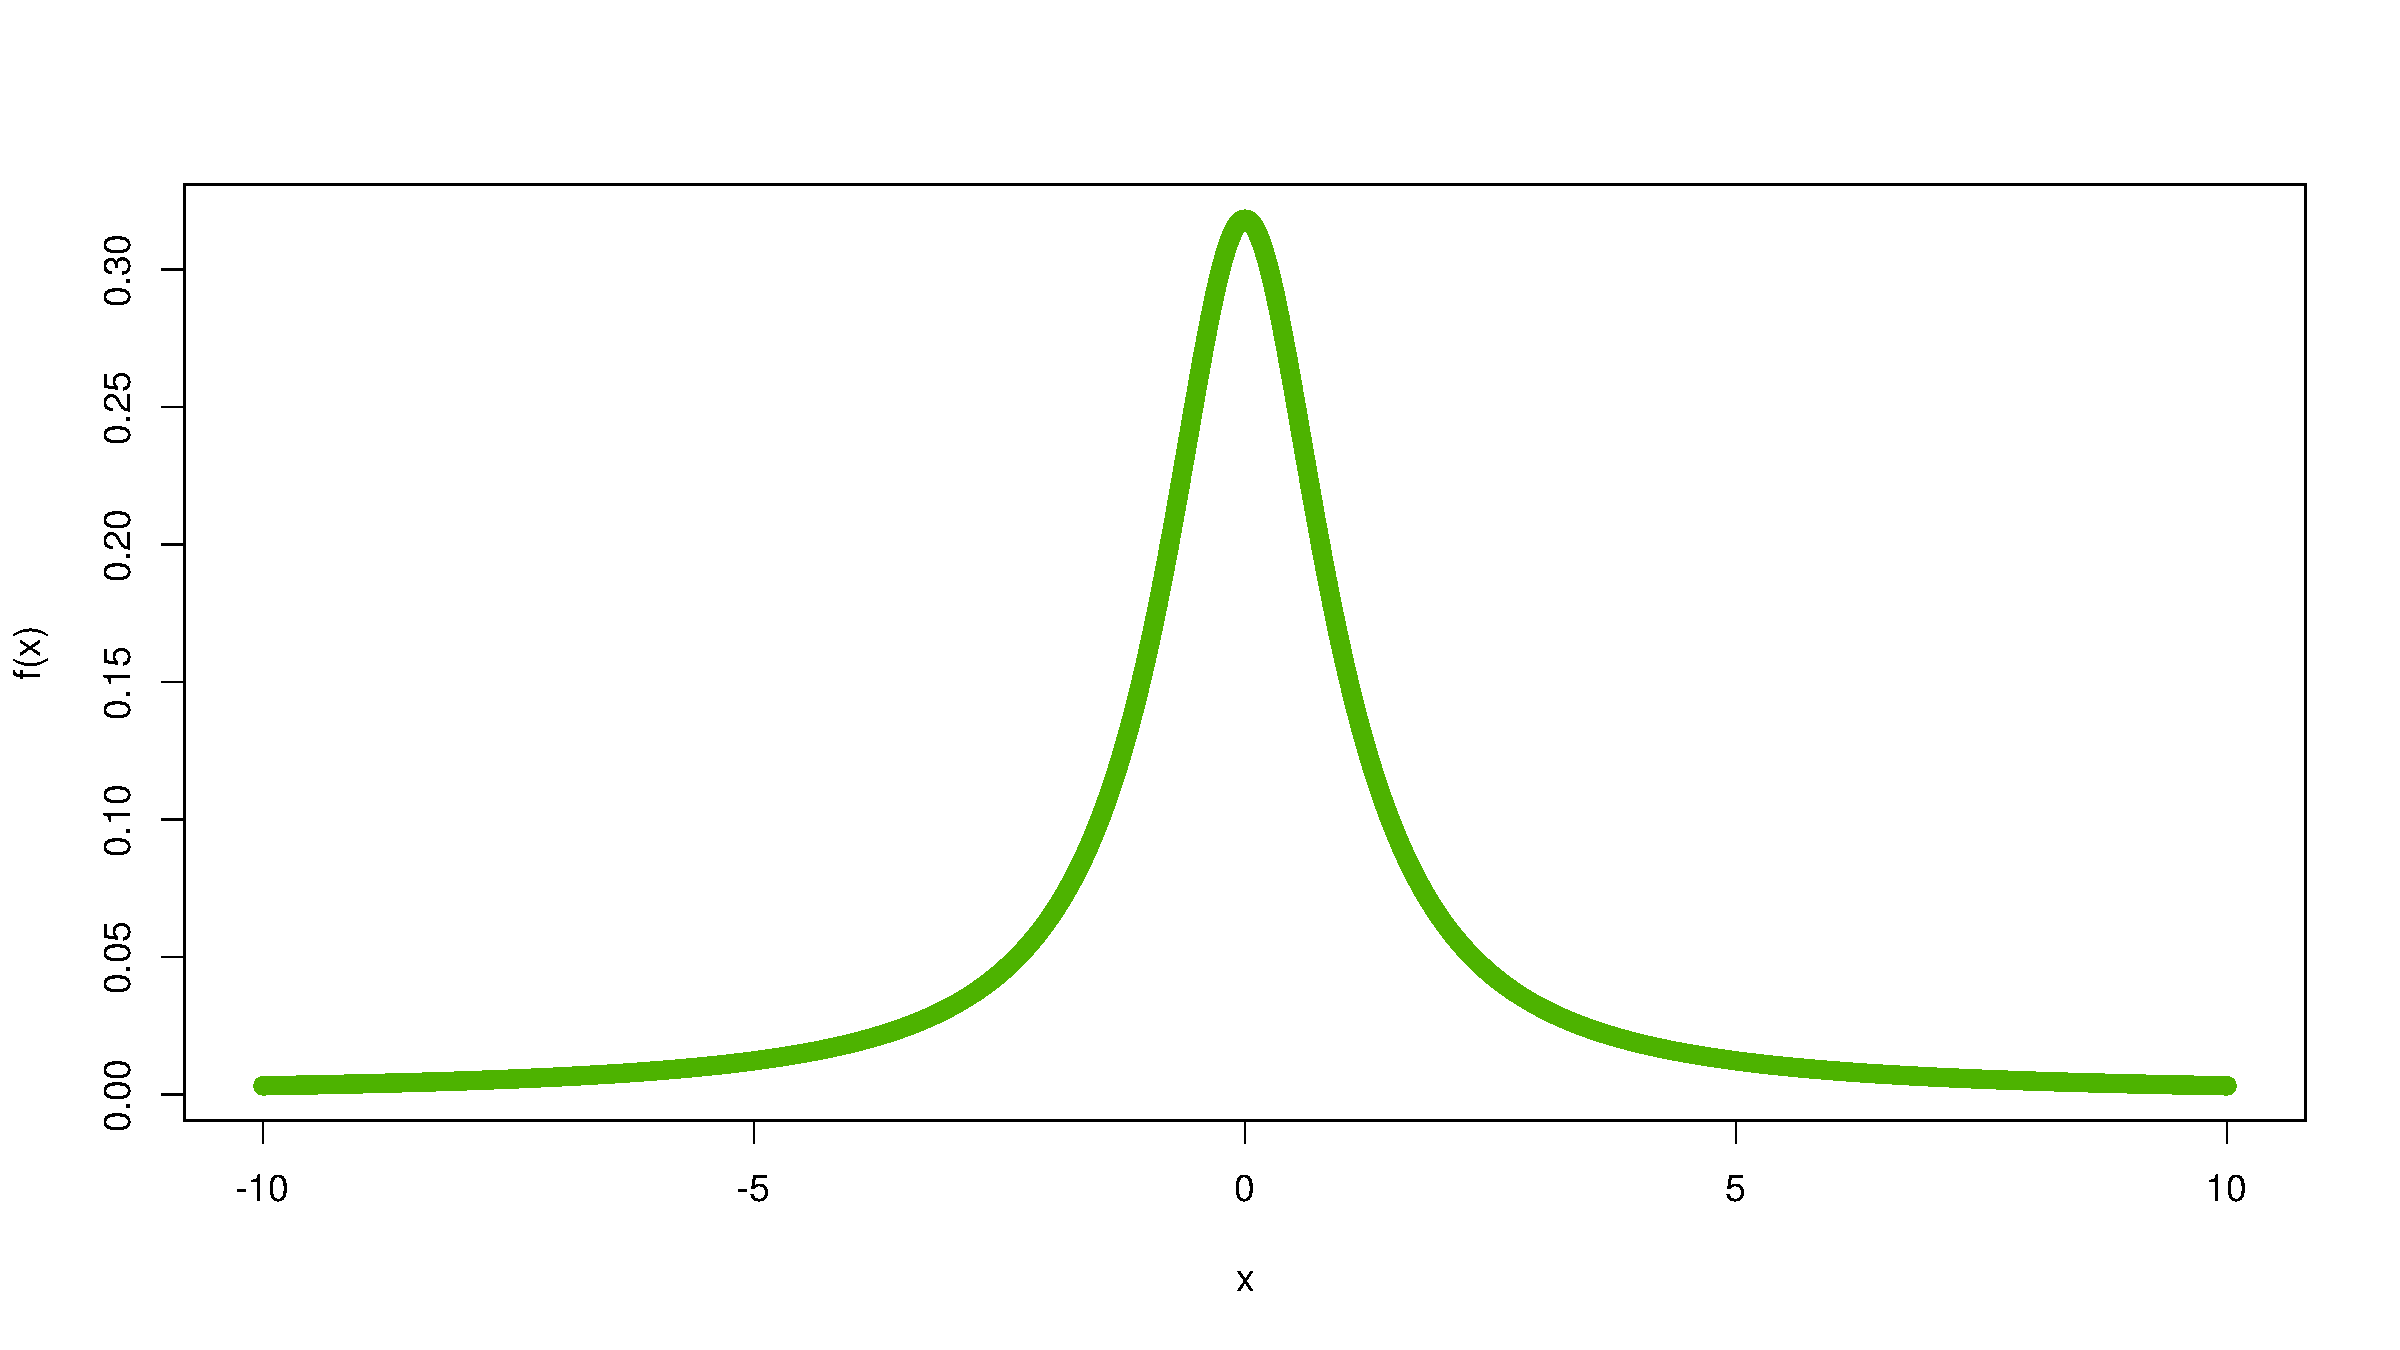
\includegraphics[width=.98\textwidth, trim={0 1cm 0 2.5cm},clip]{Immagini/Breit-Wigner.pdf}
	\label{fig:Breit-Wigner}
\end{figure}

\noindent Pertanto invertendo la relazione

$$ \xi = \frac{1}{\pi}\arctan\left[\frac{x-x_0}{\Gamma}\right] + \frac{1}{2}$$

\noindent otteniamo l'equazione desiderata:

$$\boxed{x = x_0 + \Gamma\tan\left[\pi\left(\xi-\frac{1}{2}\right)\right]}$$\\

\noindent Per generare i numeri casuali $\xi$ si è utilizzato il pacchetto \texttt{RNG} dell'ambiente statistico \texttt{R}, che permette di ottenere sequenze pseudo-random con periodo pari a $(2^{19937} - 1)$, per mezzo di un generatore di tipo "Twisted GFSR".\footnote{In particolare il pacchetto permette di eseguire svariati algoritmi per la generazione delle sequenze pseudo-random, selezionati specificando il parametro \texttt{rng.kind} nel codice.  L'opzione di default implementa l'algoritmo \emph{Marsenne-Twister}, sviluppato nel 1998 da Matsumoto e Nishimura [ACM article: \href{https://doi.org/10.1145/272991.272995}{\texttt{doi:10.1145/272991.272995}}].\\
Per maggiori dettagli sul pacchetto \texttt{RNG}: \url{https://stat.ethz.ch/R-manual/R-devel/library/base/html/Random.html}}\\

\noindent In Figura~\ref{fig:Es1A_Results} è rappresentato l'istogramma relativo a $N=10^5$ estrazioni di $x$, raggruppate in $50$ bins, con parametri Breit-Wigner $x_0 = 0$ e $\Gamma = 1$. L'ottima sovrapposizione con il grafico analitico della $f_{_{\mathrm{BW}}}(x)$ conferma la bontà del metodo implementato.\footnote{Per quanto riguarda i limiti di affidabilità dell'algoritmo proposto si tenga presente che il numero di estrazioni $N$ non dovrà mai essere comparabile con il periodo di ripetizione del generatore pseudo-random adoperato.}\\

\begin{figure}
	\centering
	\caption{Uno degli istogrammi generati a confronto con il grafico analitico della distribuzione.}
	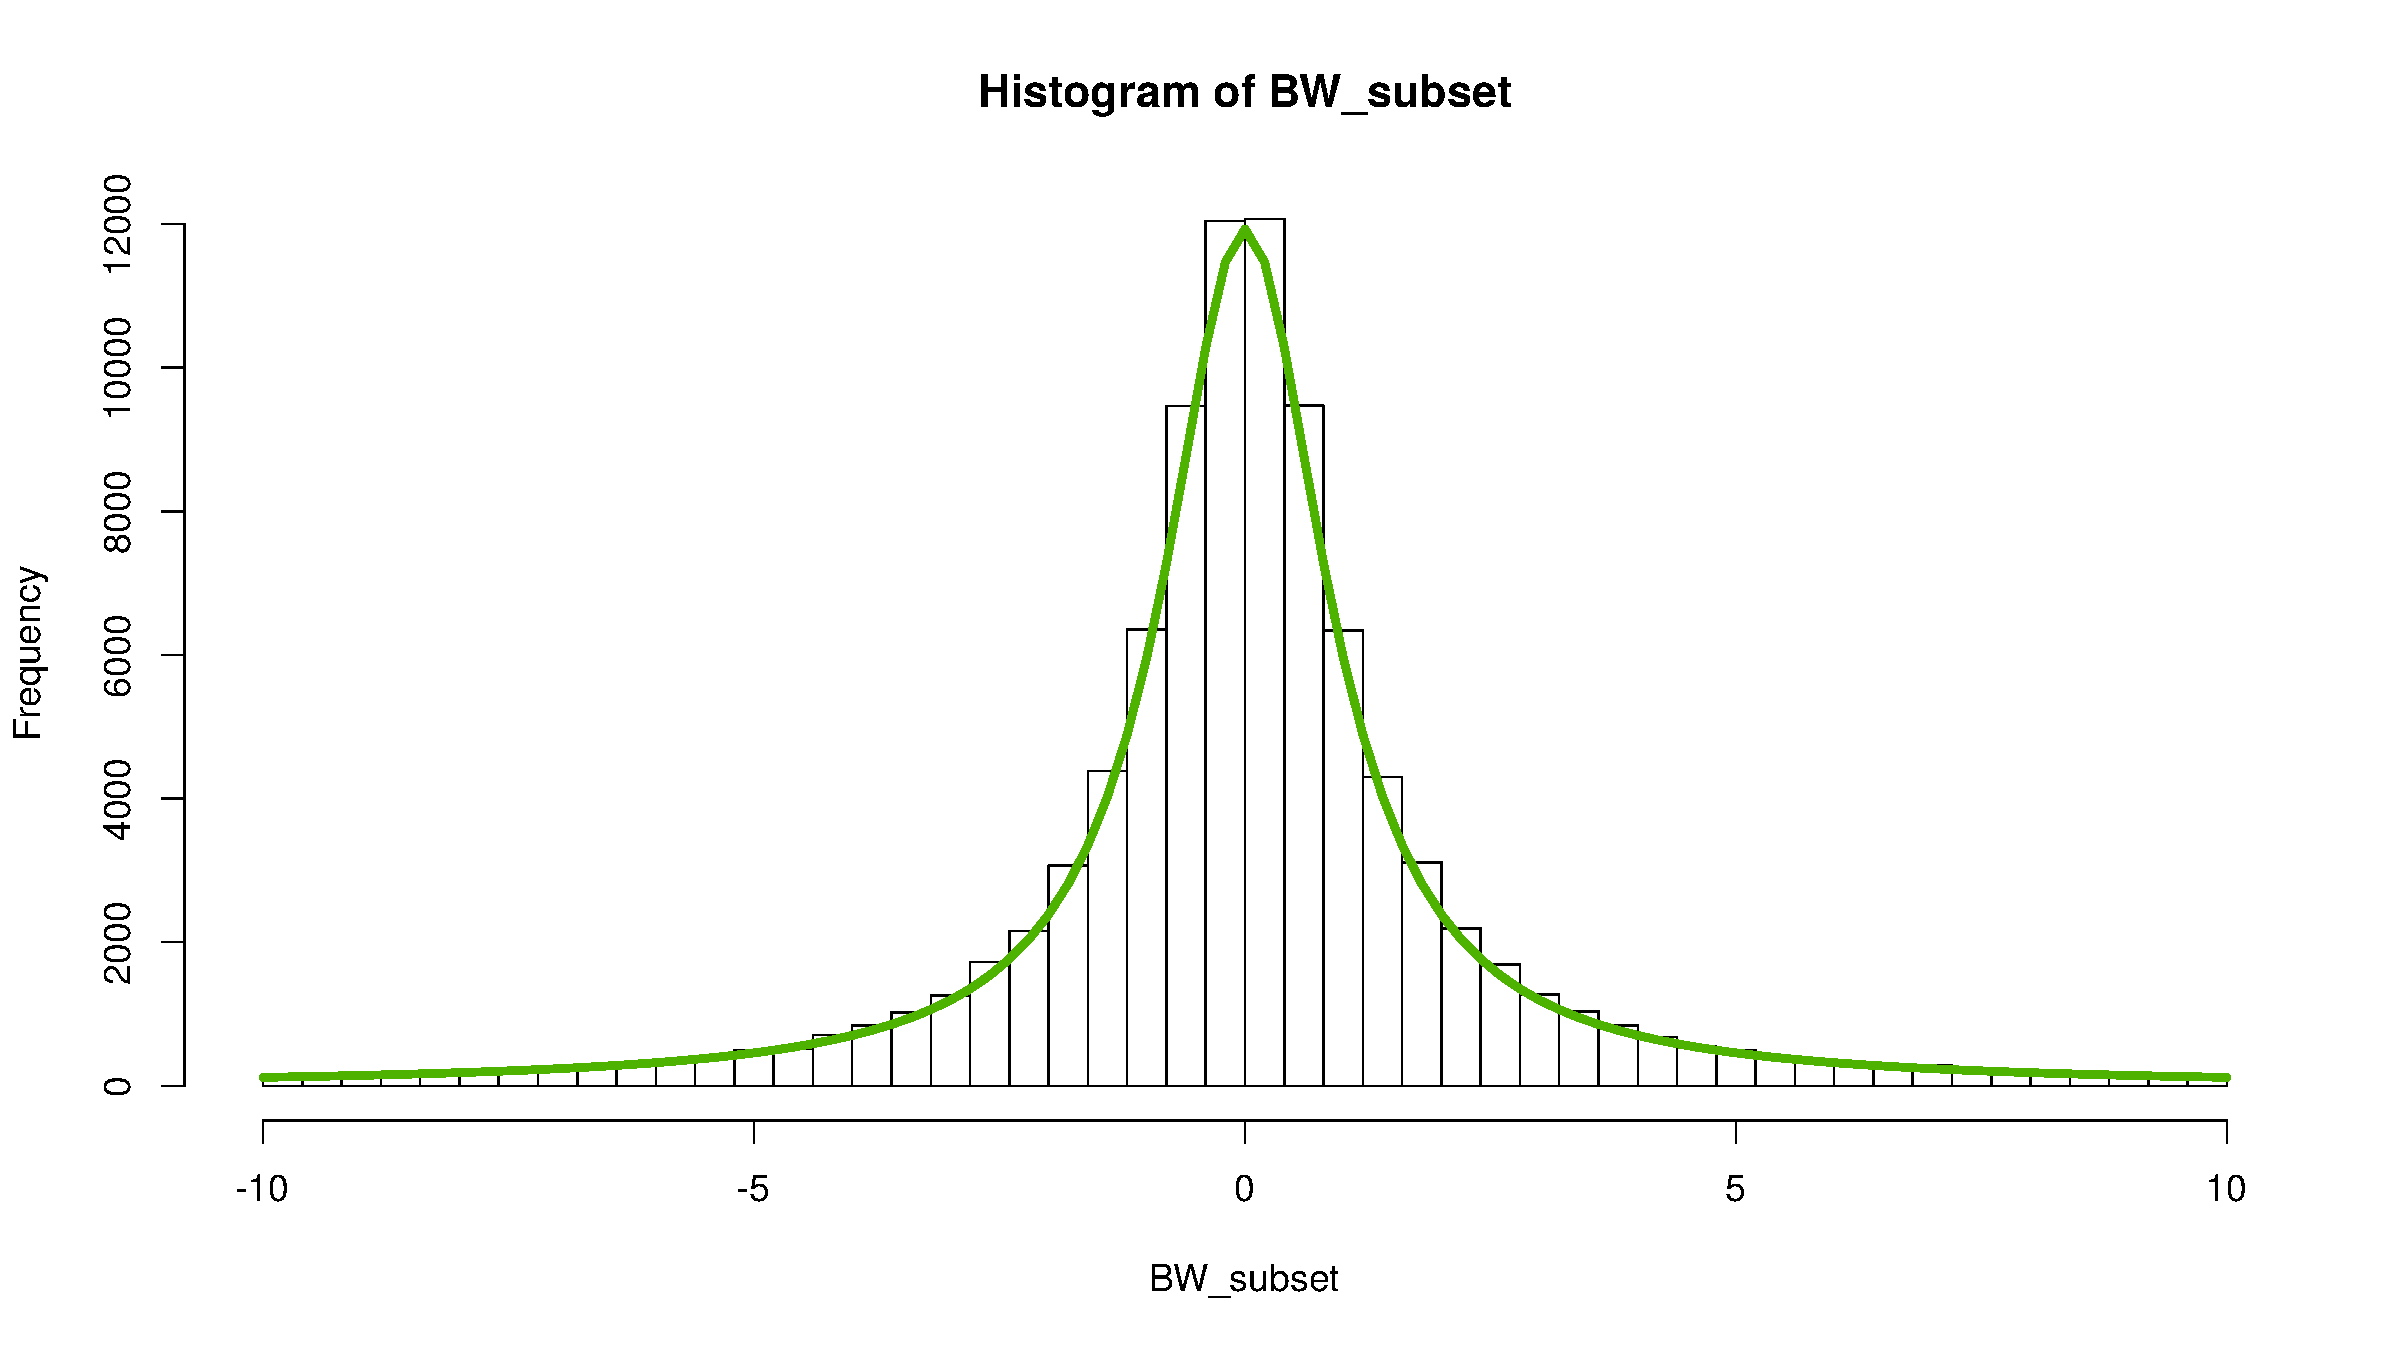
\includegraphics[width=\textwidth, trim={0 1cm 0 2.3cm},clip]{Immagini/BW_histogram.pdf}
	\label{fig:Es1A_Results}
\end{figure}

\noindent Di seguito viene riportato il listato del codice \texttt{R} utilizzato:

\begin{lstlisting}[language=R, style=Rstyle, caption=\texttt{R} code for Exercise 1/A (to generate a Breit-Wigner histogram), xleftmargin=.02\textwidth]
# Entering here the desired Breit-Wigner parameters:
x0 = 0
HWHM = 1

# Setting here an appropriate x domain (as a linear spaced vector)
x = seq(-10, 10, by = 0.04) # Note that "by" fixes the number of bins

# Defining the Breit-Wigner function
f_x = HWHM / (pi*HWHM^2 + pi*(x-x0)^2)

# Plotting and saving a graph of the function
cairo_pdf('Breit-Wigner.pdf', width = 16, height = 9, pointsize = 18)
mycolor = rgb(0.3, 0.7, 0)
plot(x, f_x, xlab='x', ylab='f(x)', col=mycolor)
dev.off()

# Extracting the required N uniform random numbers (N is a parameter of choice)
N = 10^5
uniform_set = runif(N, 0, 1) 

# Using inverse-cumulant equation to get Breit-Wigner dataset
BW_set = x0 + HWHM*tan(pi*(uniform_set-1/2))
	
# Defining histogram range and bins from x vector
hist_range = range(x)
bins = x

# Retrieving a proper subset of Breit-Wigner data 
BW_subset = subset(BW_set, BW_set <= max(hist_range) & BW_set >= min(hist_range))

# Plotting and saving the histogram of Breit-Wigner dataset (with analitical check)
myhistogram = hist(BW_subset, bins)
A = (myhistogram$counts / myhistogram$density)[1] # Normalization factor
cairo_pdf('BW_histogram.pdf', width = 16, height = 9, pointsize = 18)
plot(myhistogram)
curve(A*dcauchy(x,location=x0,scale=HWHM,log=FALSE), lwd=5, add=TRUE,  col=mycolor)
dev.off()
\end{lstlisting}

\noindent Infine risulta interessante osservare come all'aumentare del numero di bin, fissato $N=10^5$, aumenti il "rumore" nell'istogramma prodotto (Cfr. Figura~\ref{fig:Breit-Wigner_BINS}). Ciò è del tutto ragionevole poiché più sono i bin e più sarà piccolo il campione su cui mediamo il valore da assegnare a ciascun bin. Possiamo quindi concludere che, fissato di converso il numero di bin che ci interessa, riprodurremo meglio la distribuzione tanti più saranno i numeri generati, come ci si aspetta. Una verifica concreta dell'equivalenza di queste due affermazioni si ha osservando la Figura~\ref{fig:Breit-WIgner_N}, che confronta due istogrammi con medesimo numero di bin ($500$) ma relativi rispettivamente a $10^5$ e $10^6$ eventi generati. Tutto ciò costituisce una verifica empirica del \textsl{Teorema del Limite Centrale}.

\captionsetup*[subfigure]{position=bottom}
\begin{figure}
	\centering
	\caption{Istogrammi generati per $N=10^5$ eventi, distribuiti in bin di numero crescente.}
	\subfloat[]{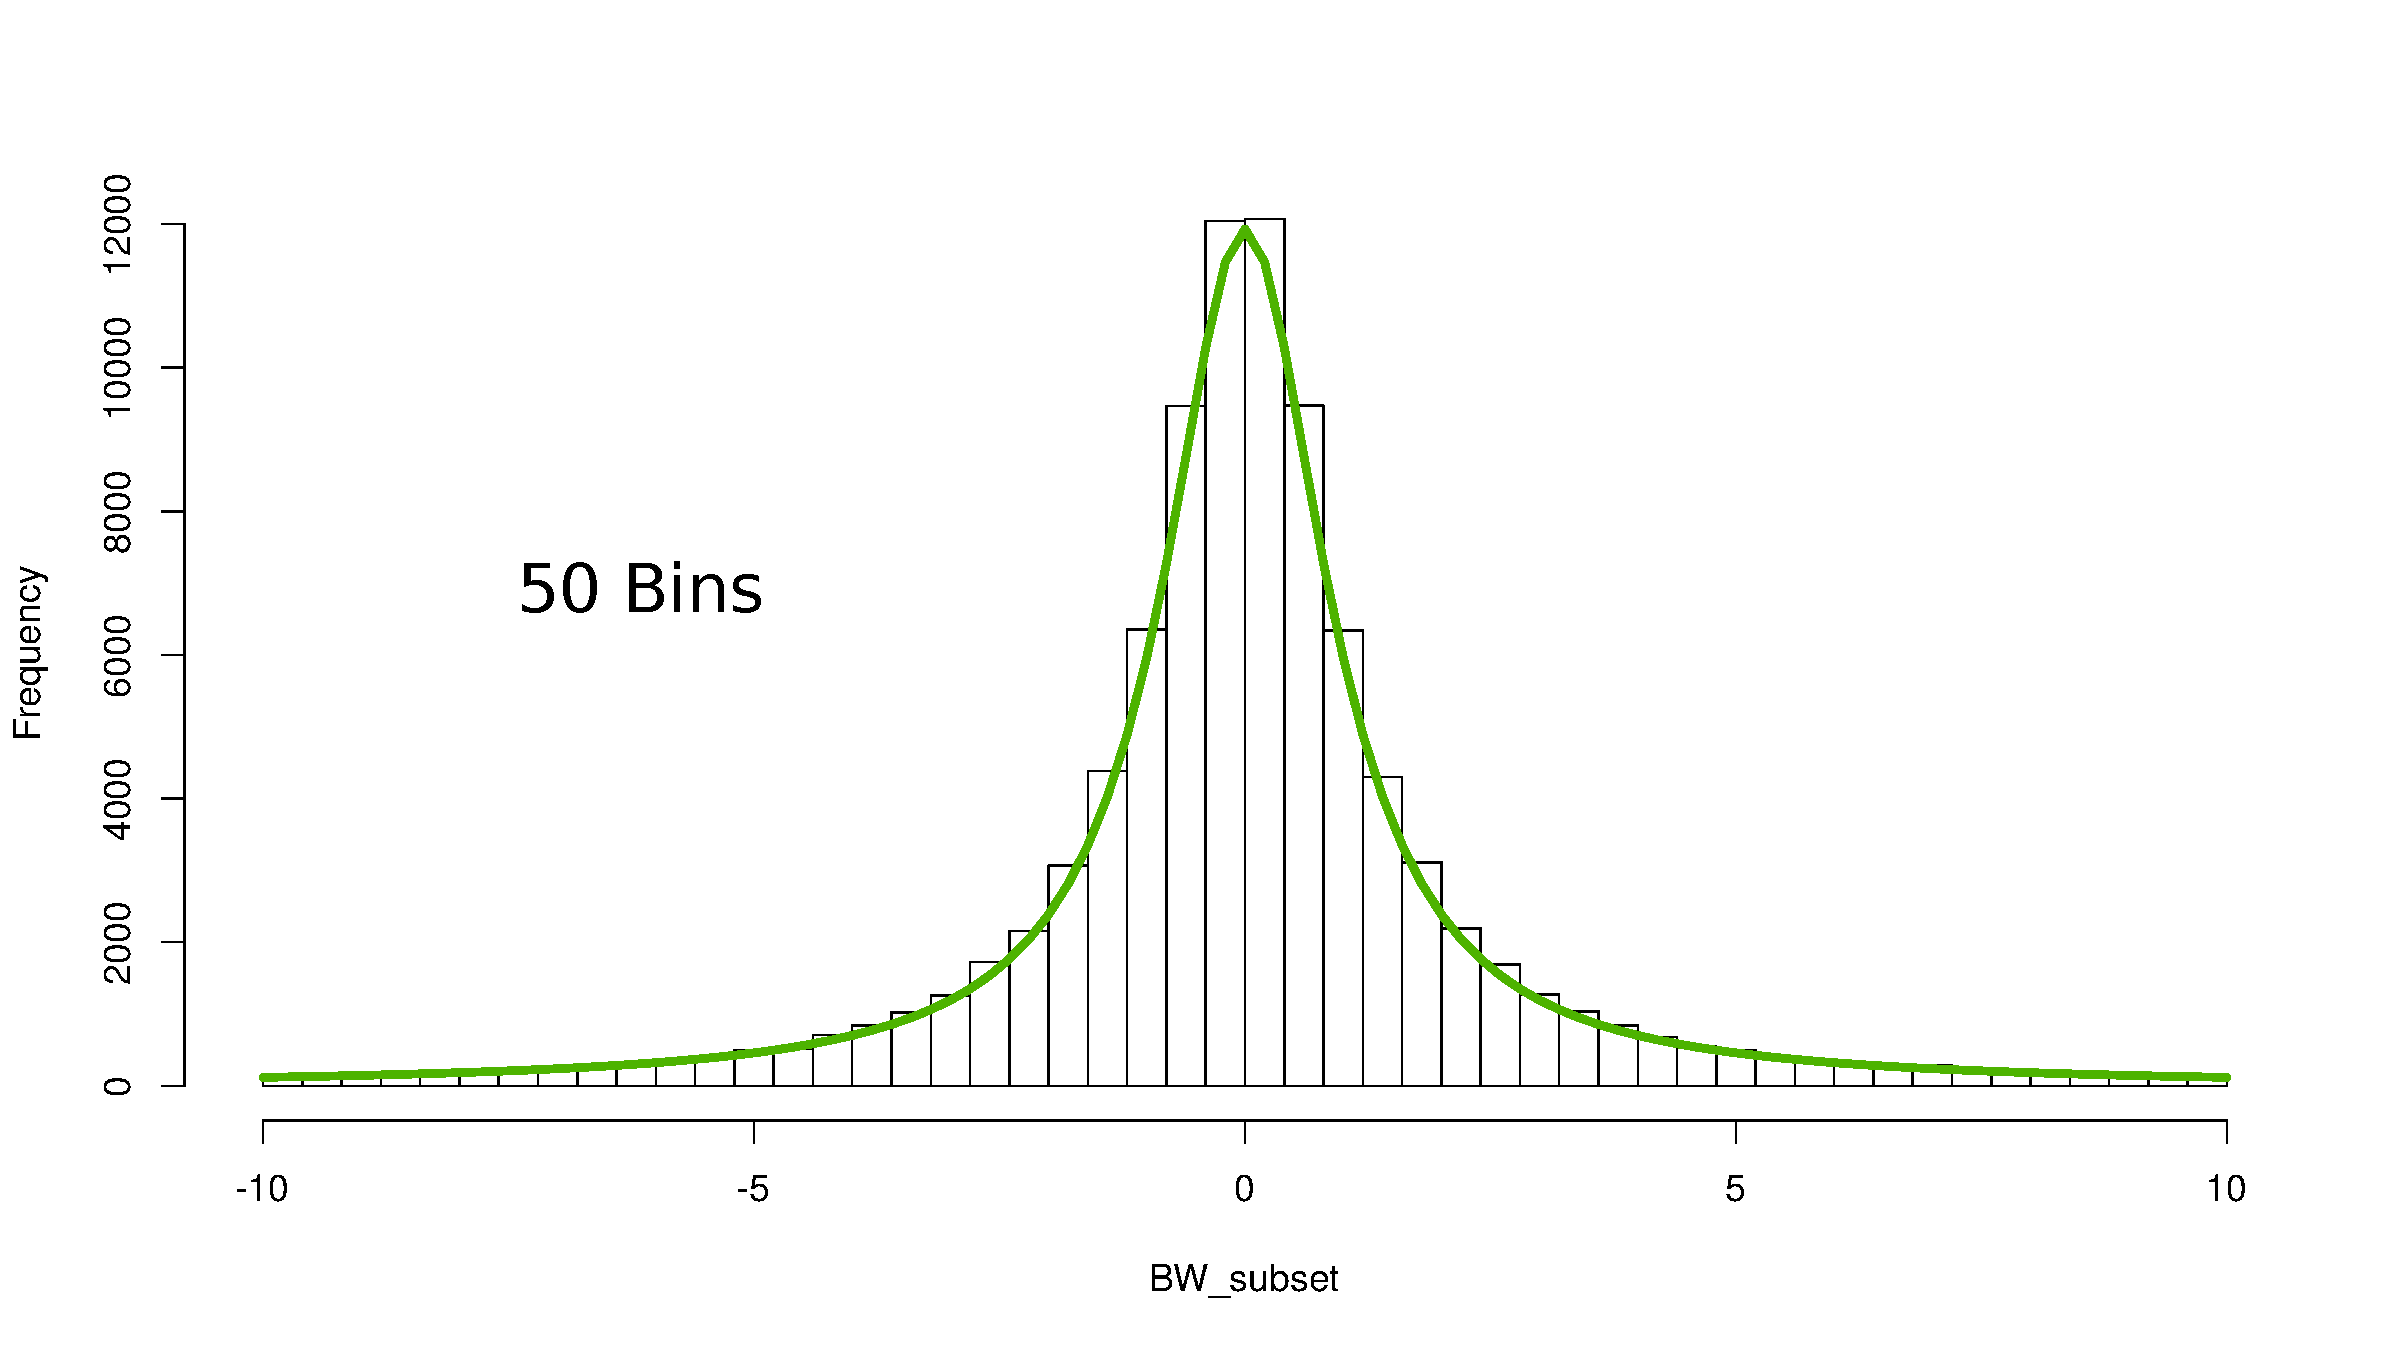
\includegraphics[width = 2.9in]{Immagini/BW_histogram_50bins.pdf}} 
	\subfloat[]{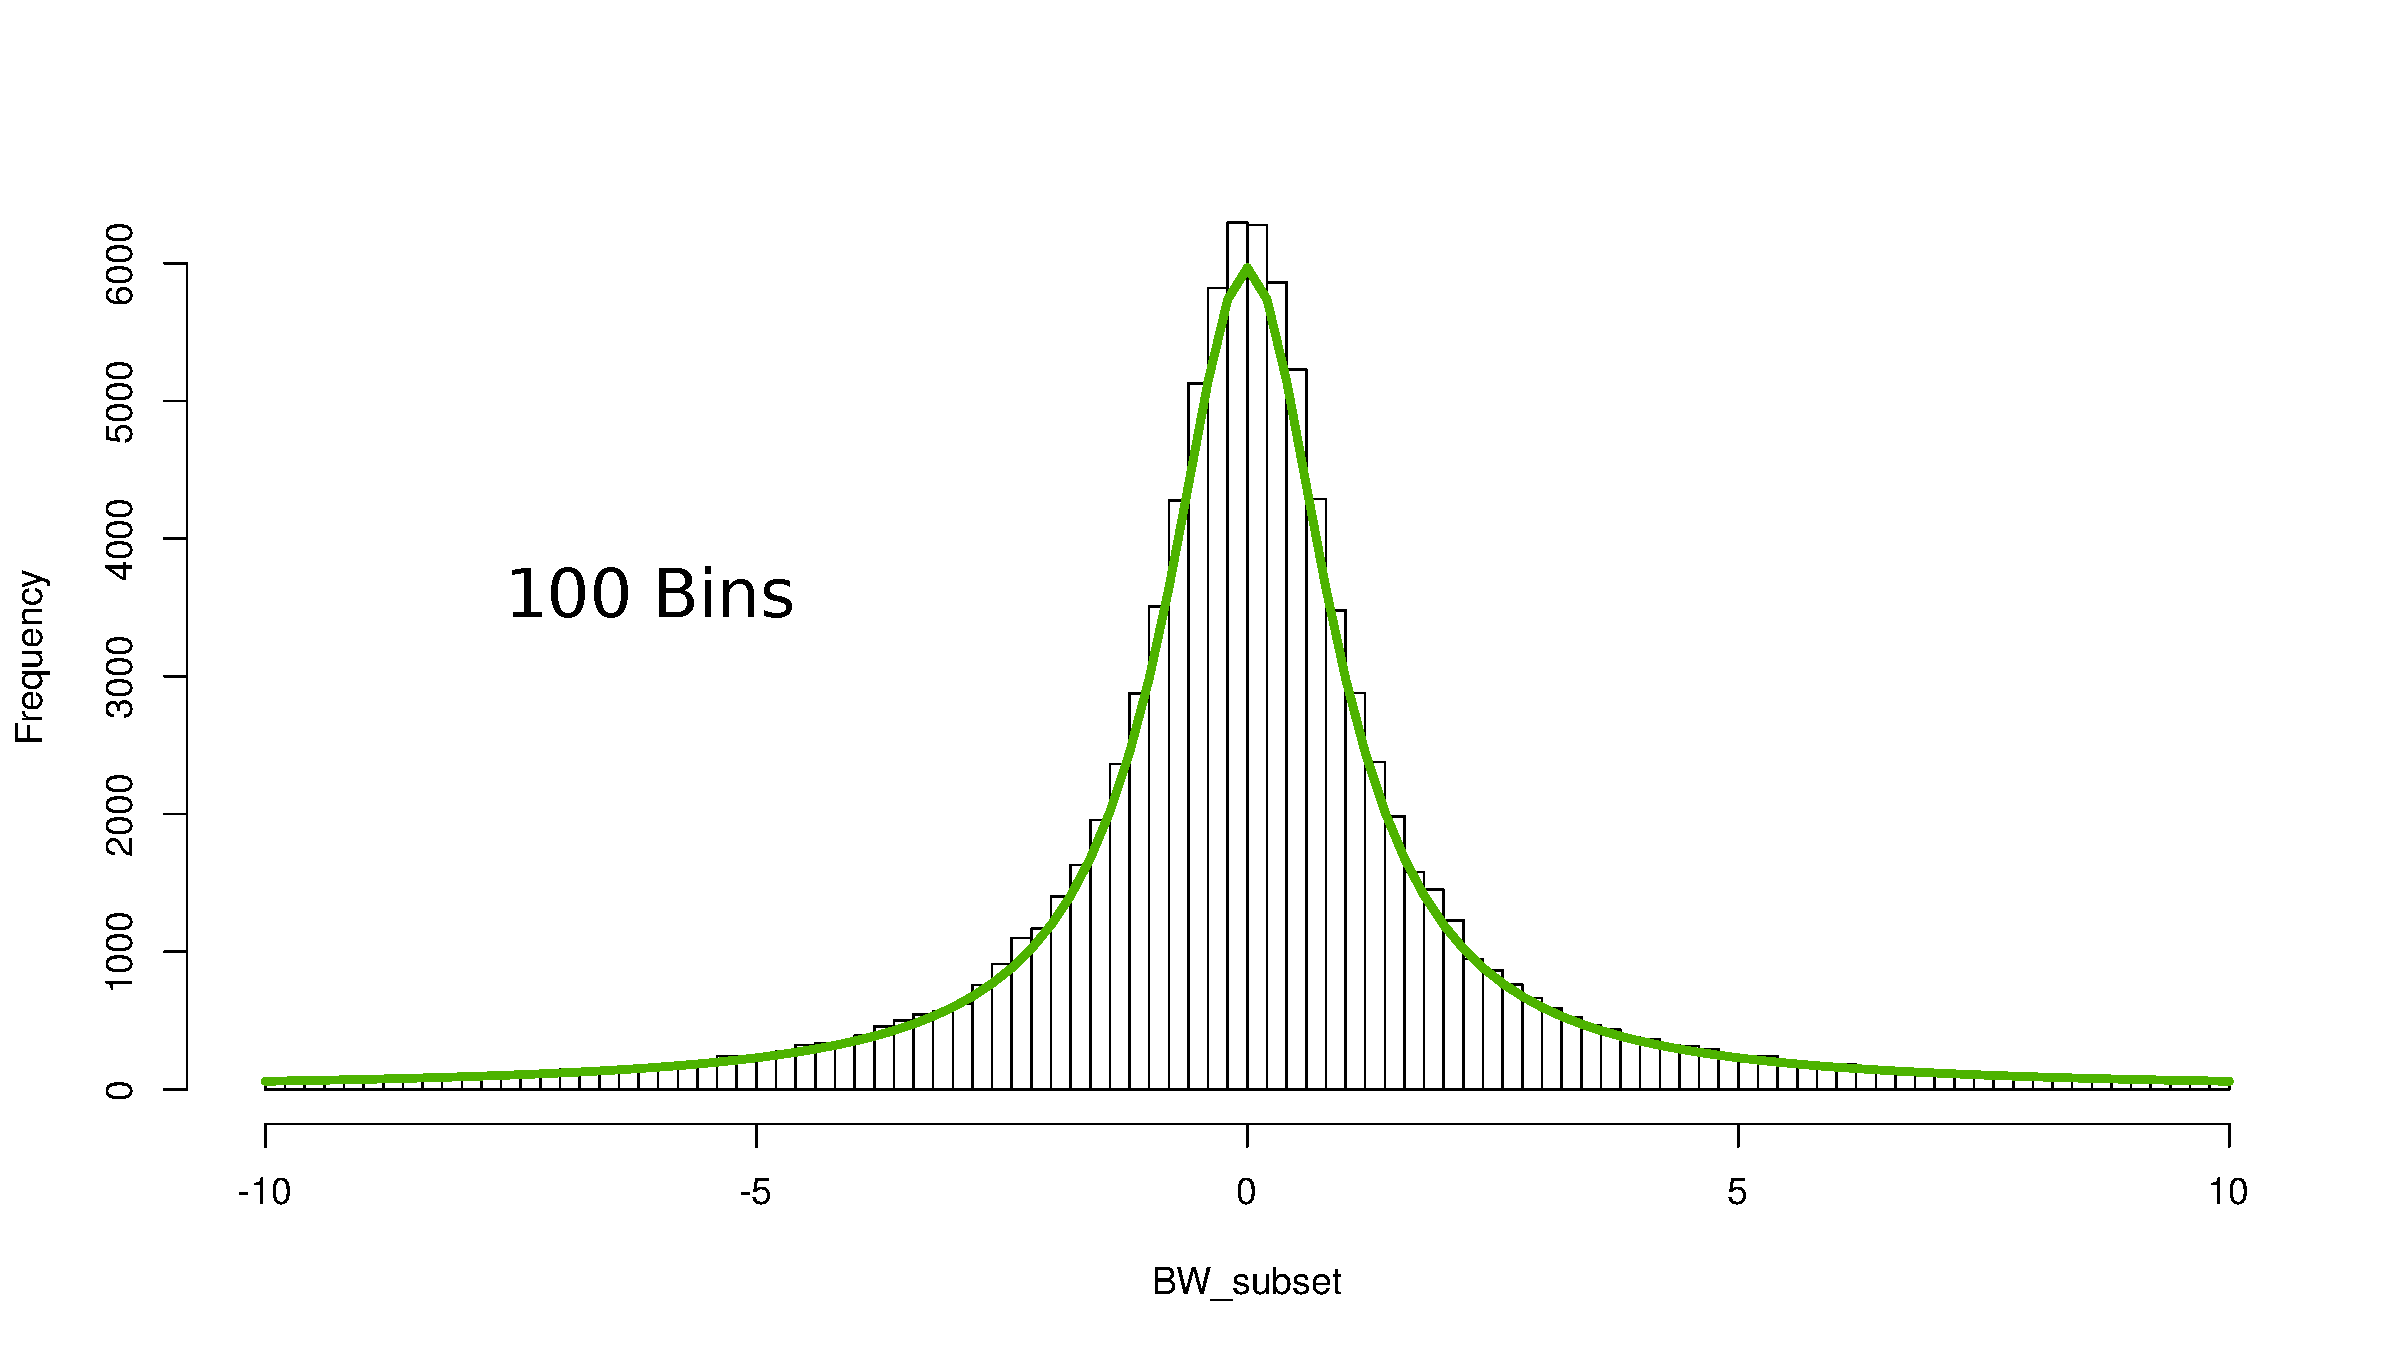
\includegraphics[width = 2.9in]{Immagini/BW_histogram_100bins.pdf}}\\
	\subfloat[]{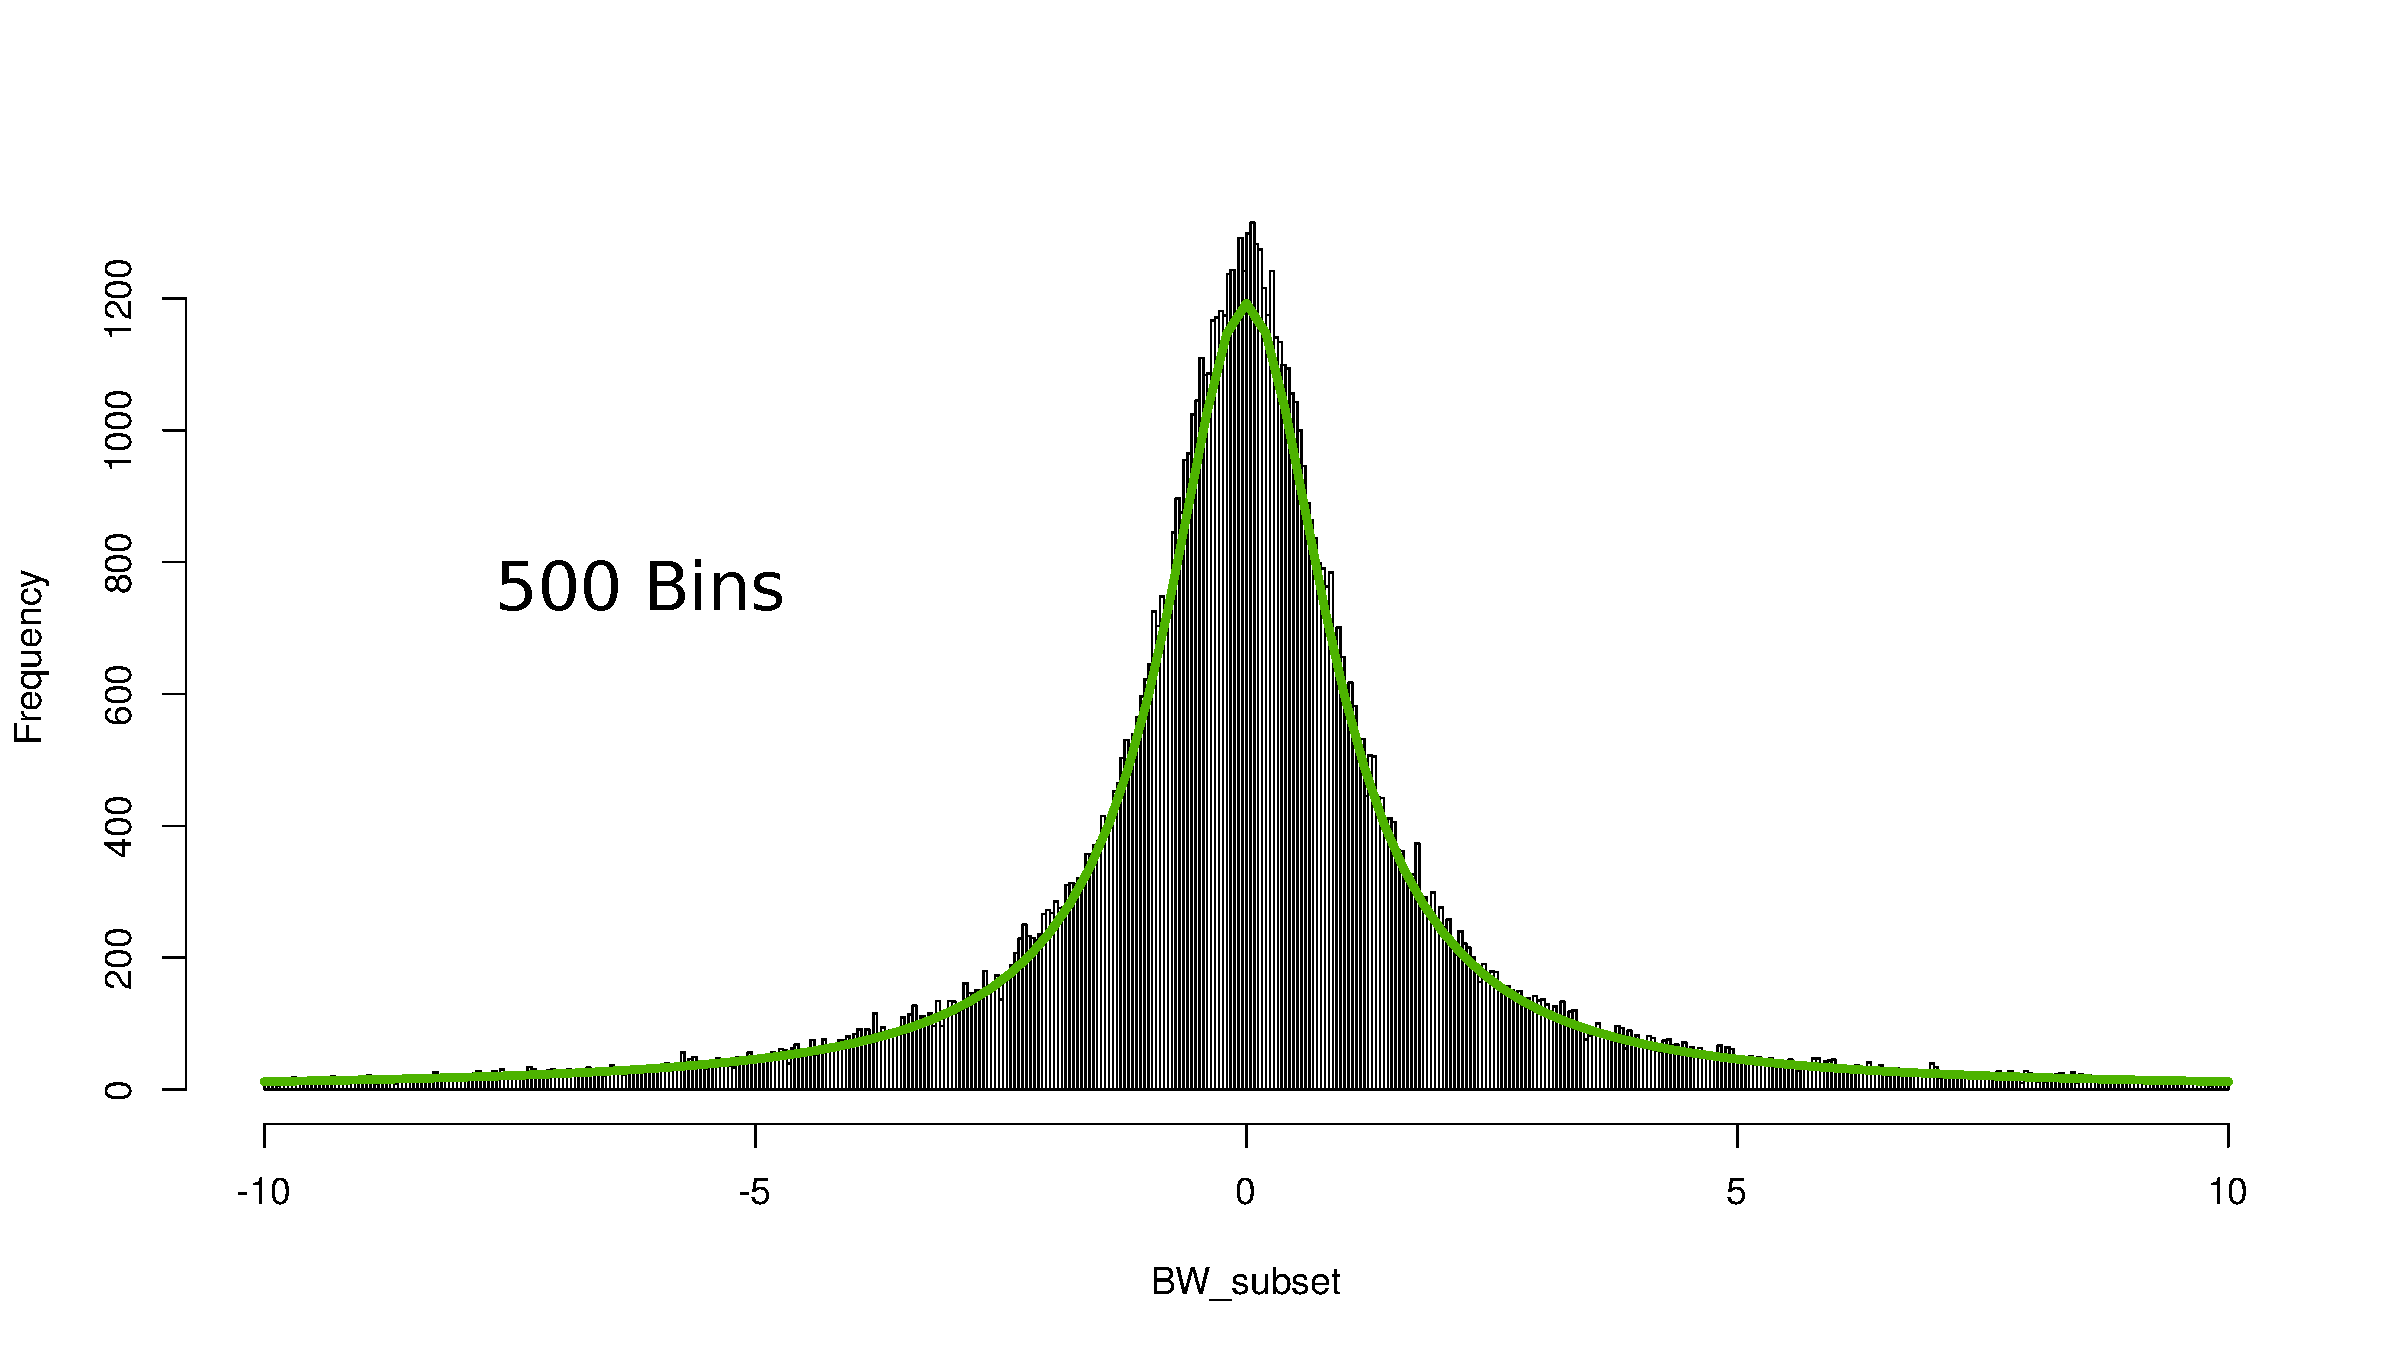
\includegraphics[width = 2.9in]{Immagini/BW_histogram_500bins.pdf}}
	\subfloat[]{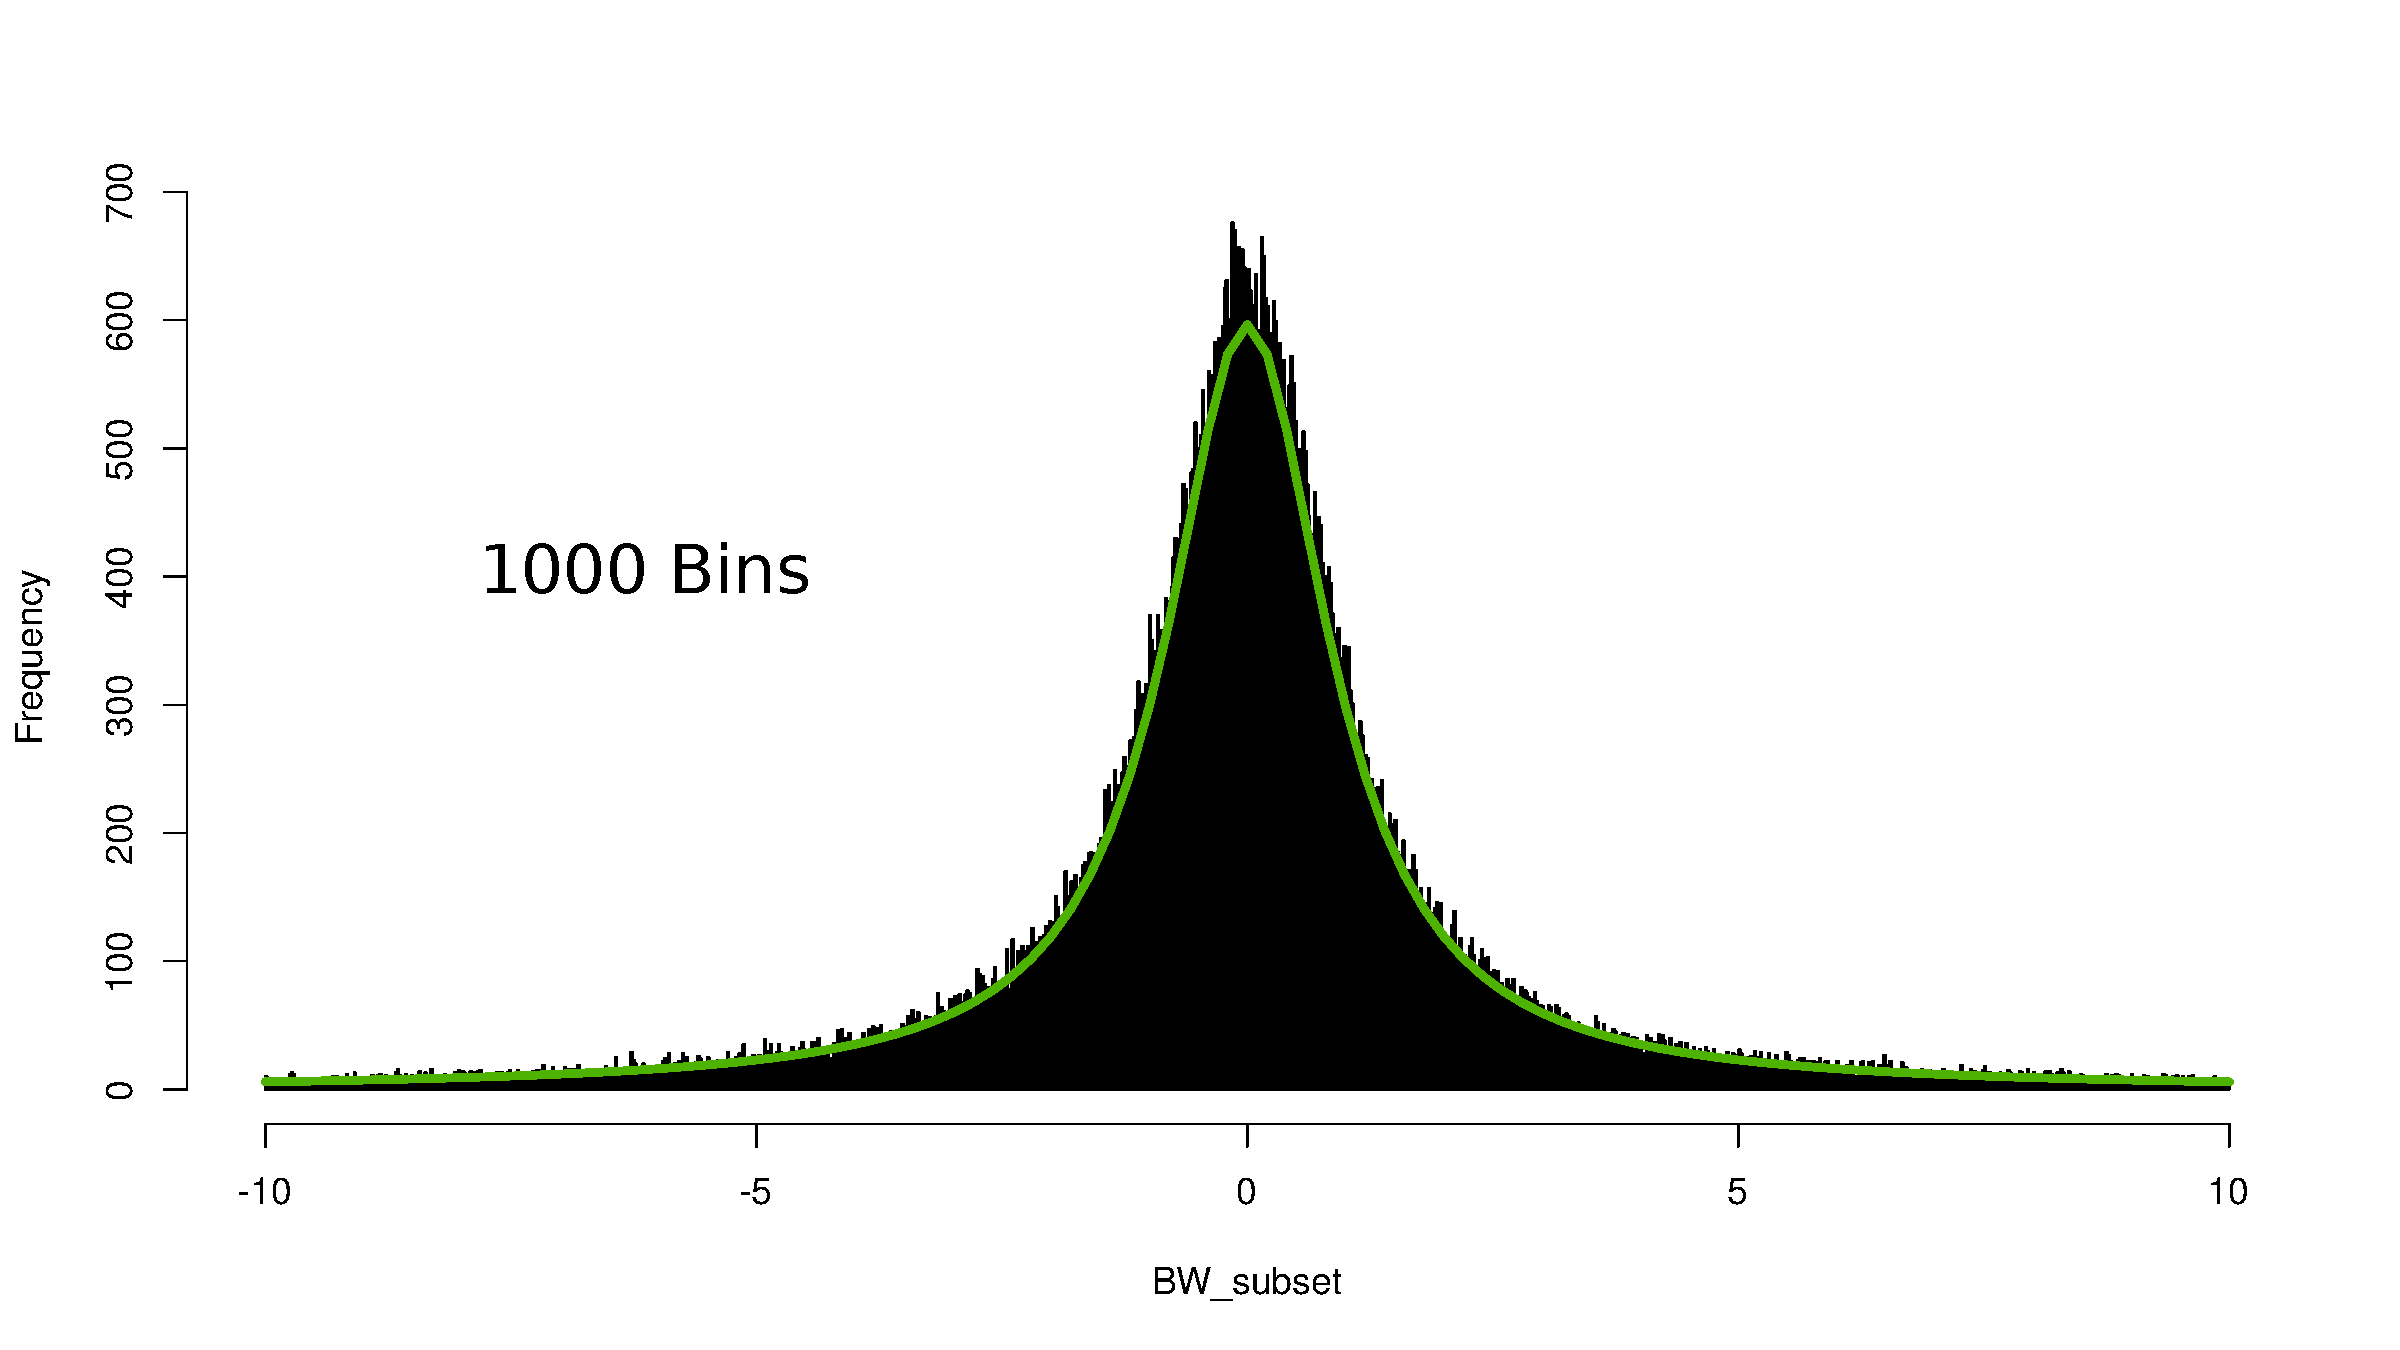
\includegraphics[width = 2.9in]{Immagini/BW_histogram_1000bins.pdf}} \\
	\subfloat[]{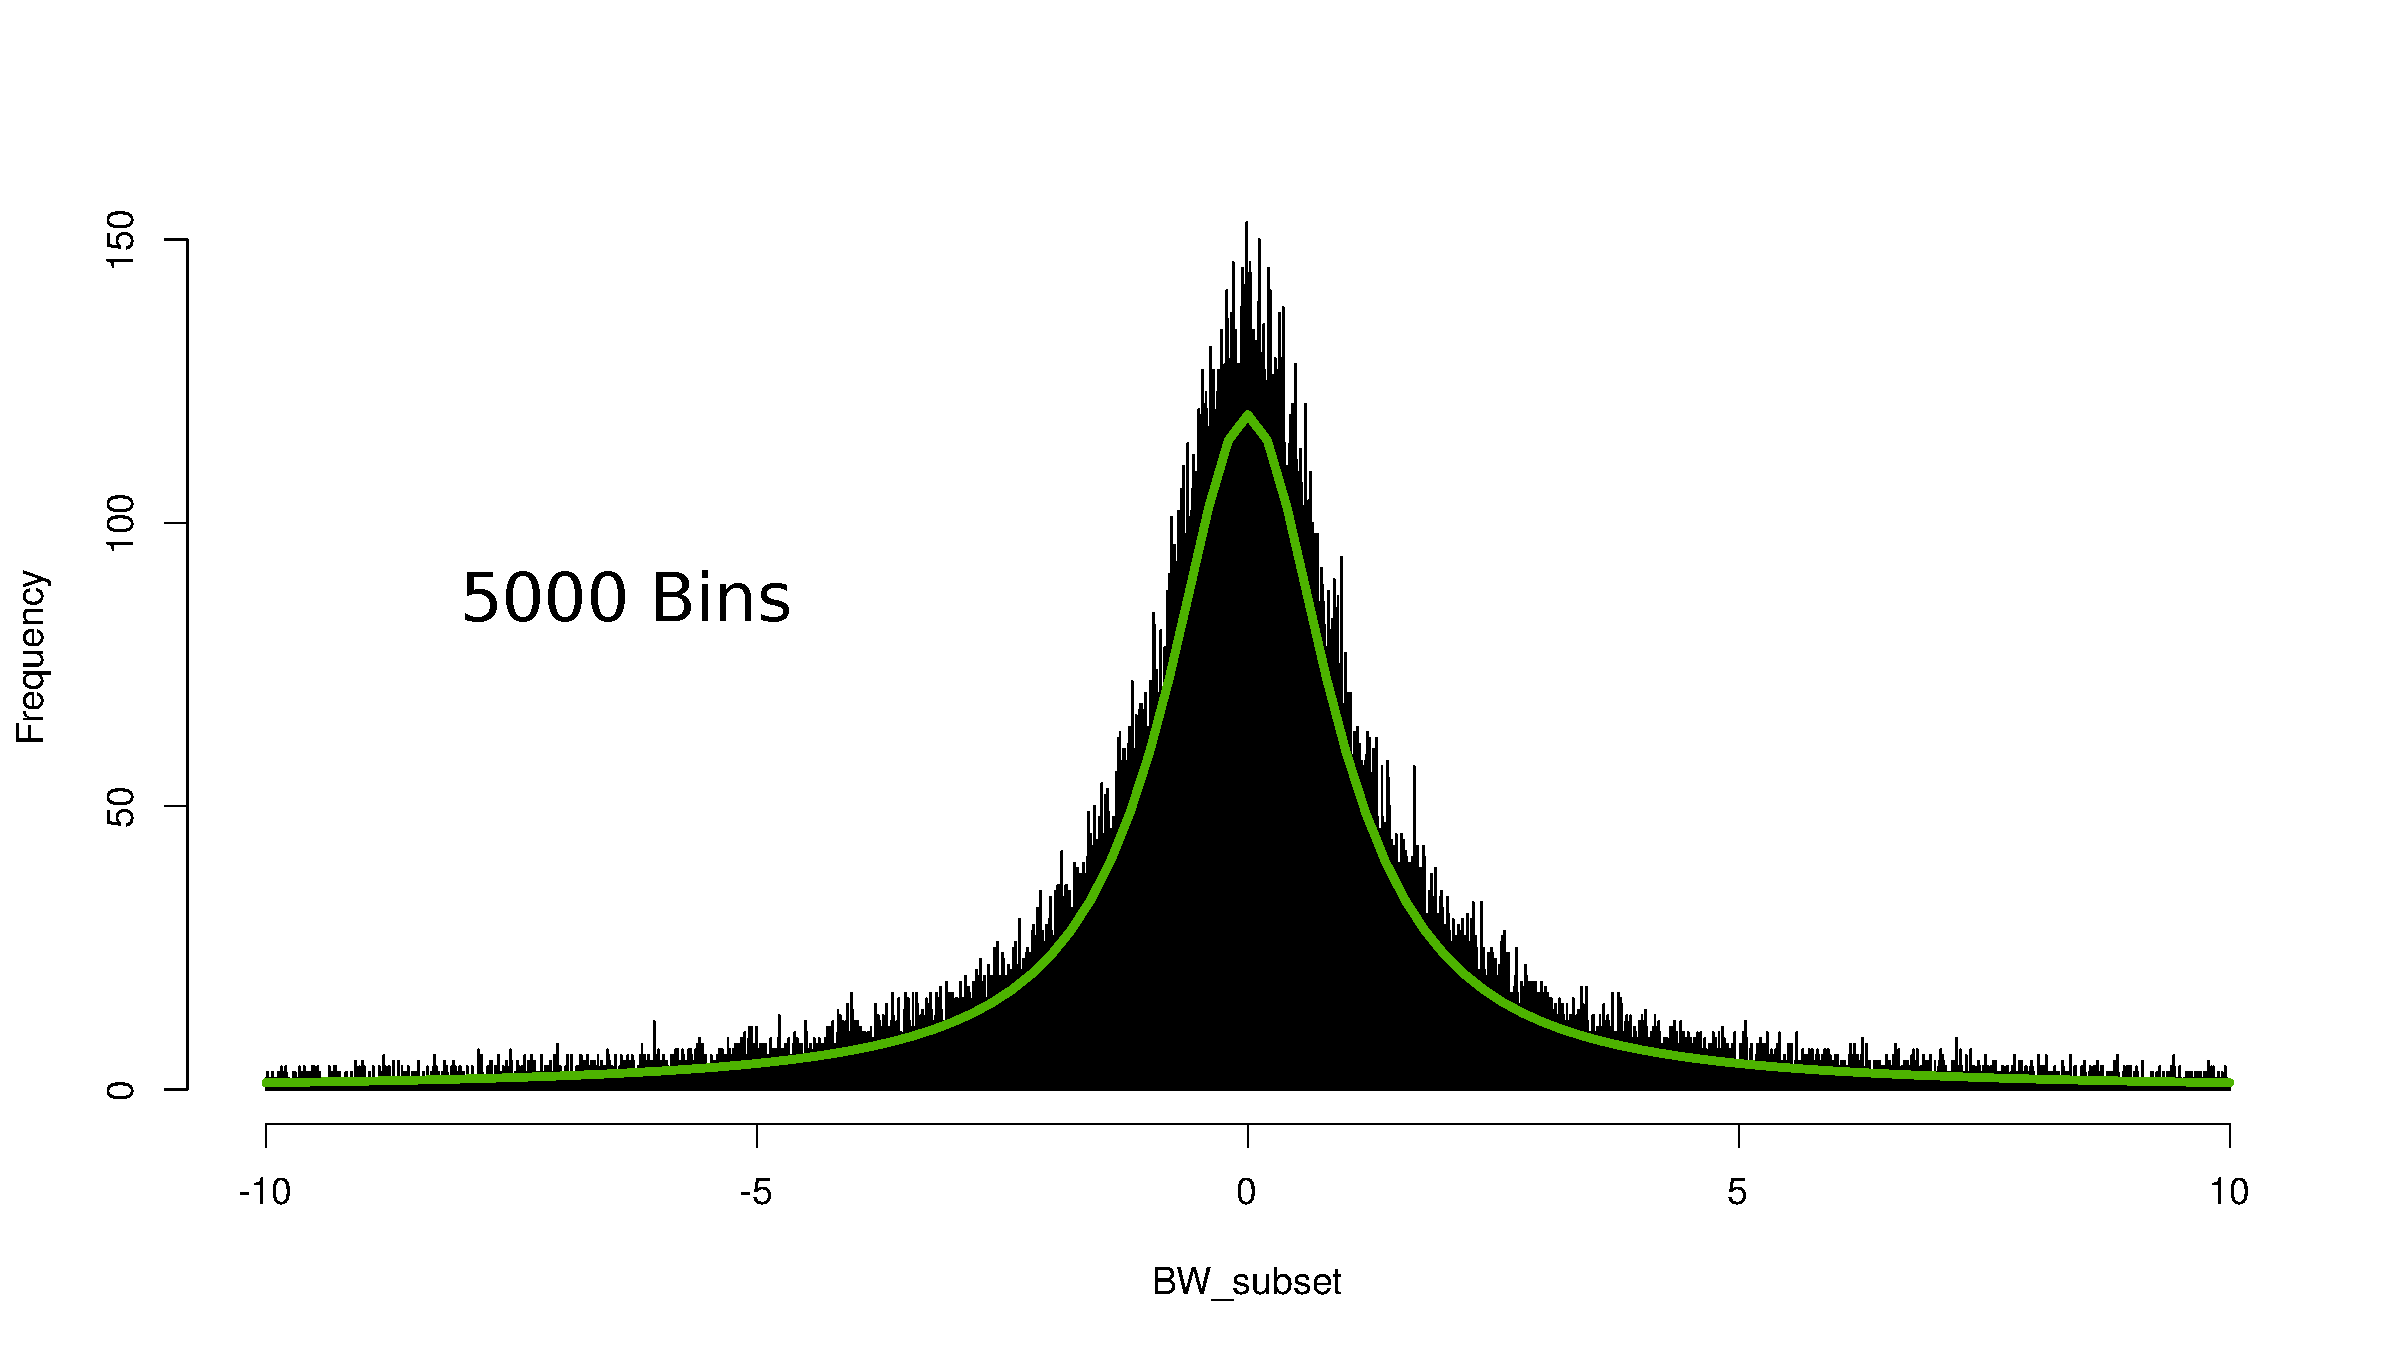
\includegraphics[width = 2.9in]{Immagini/BW_histogram_5000bins.pdf}}
	\subfloat[]{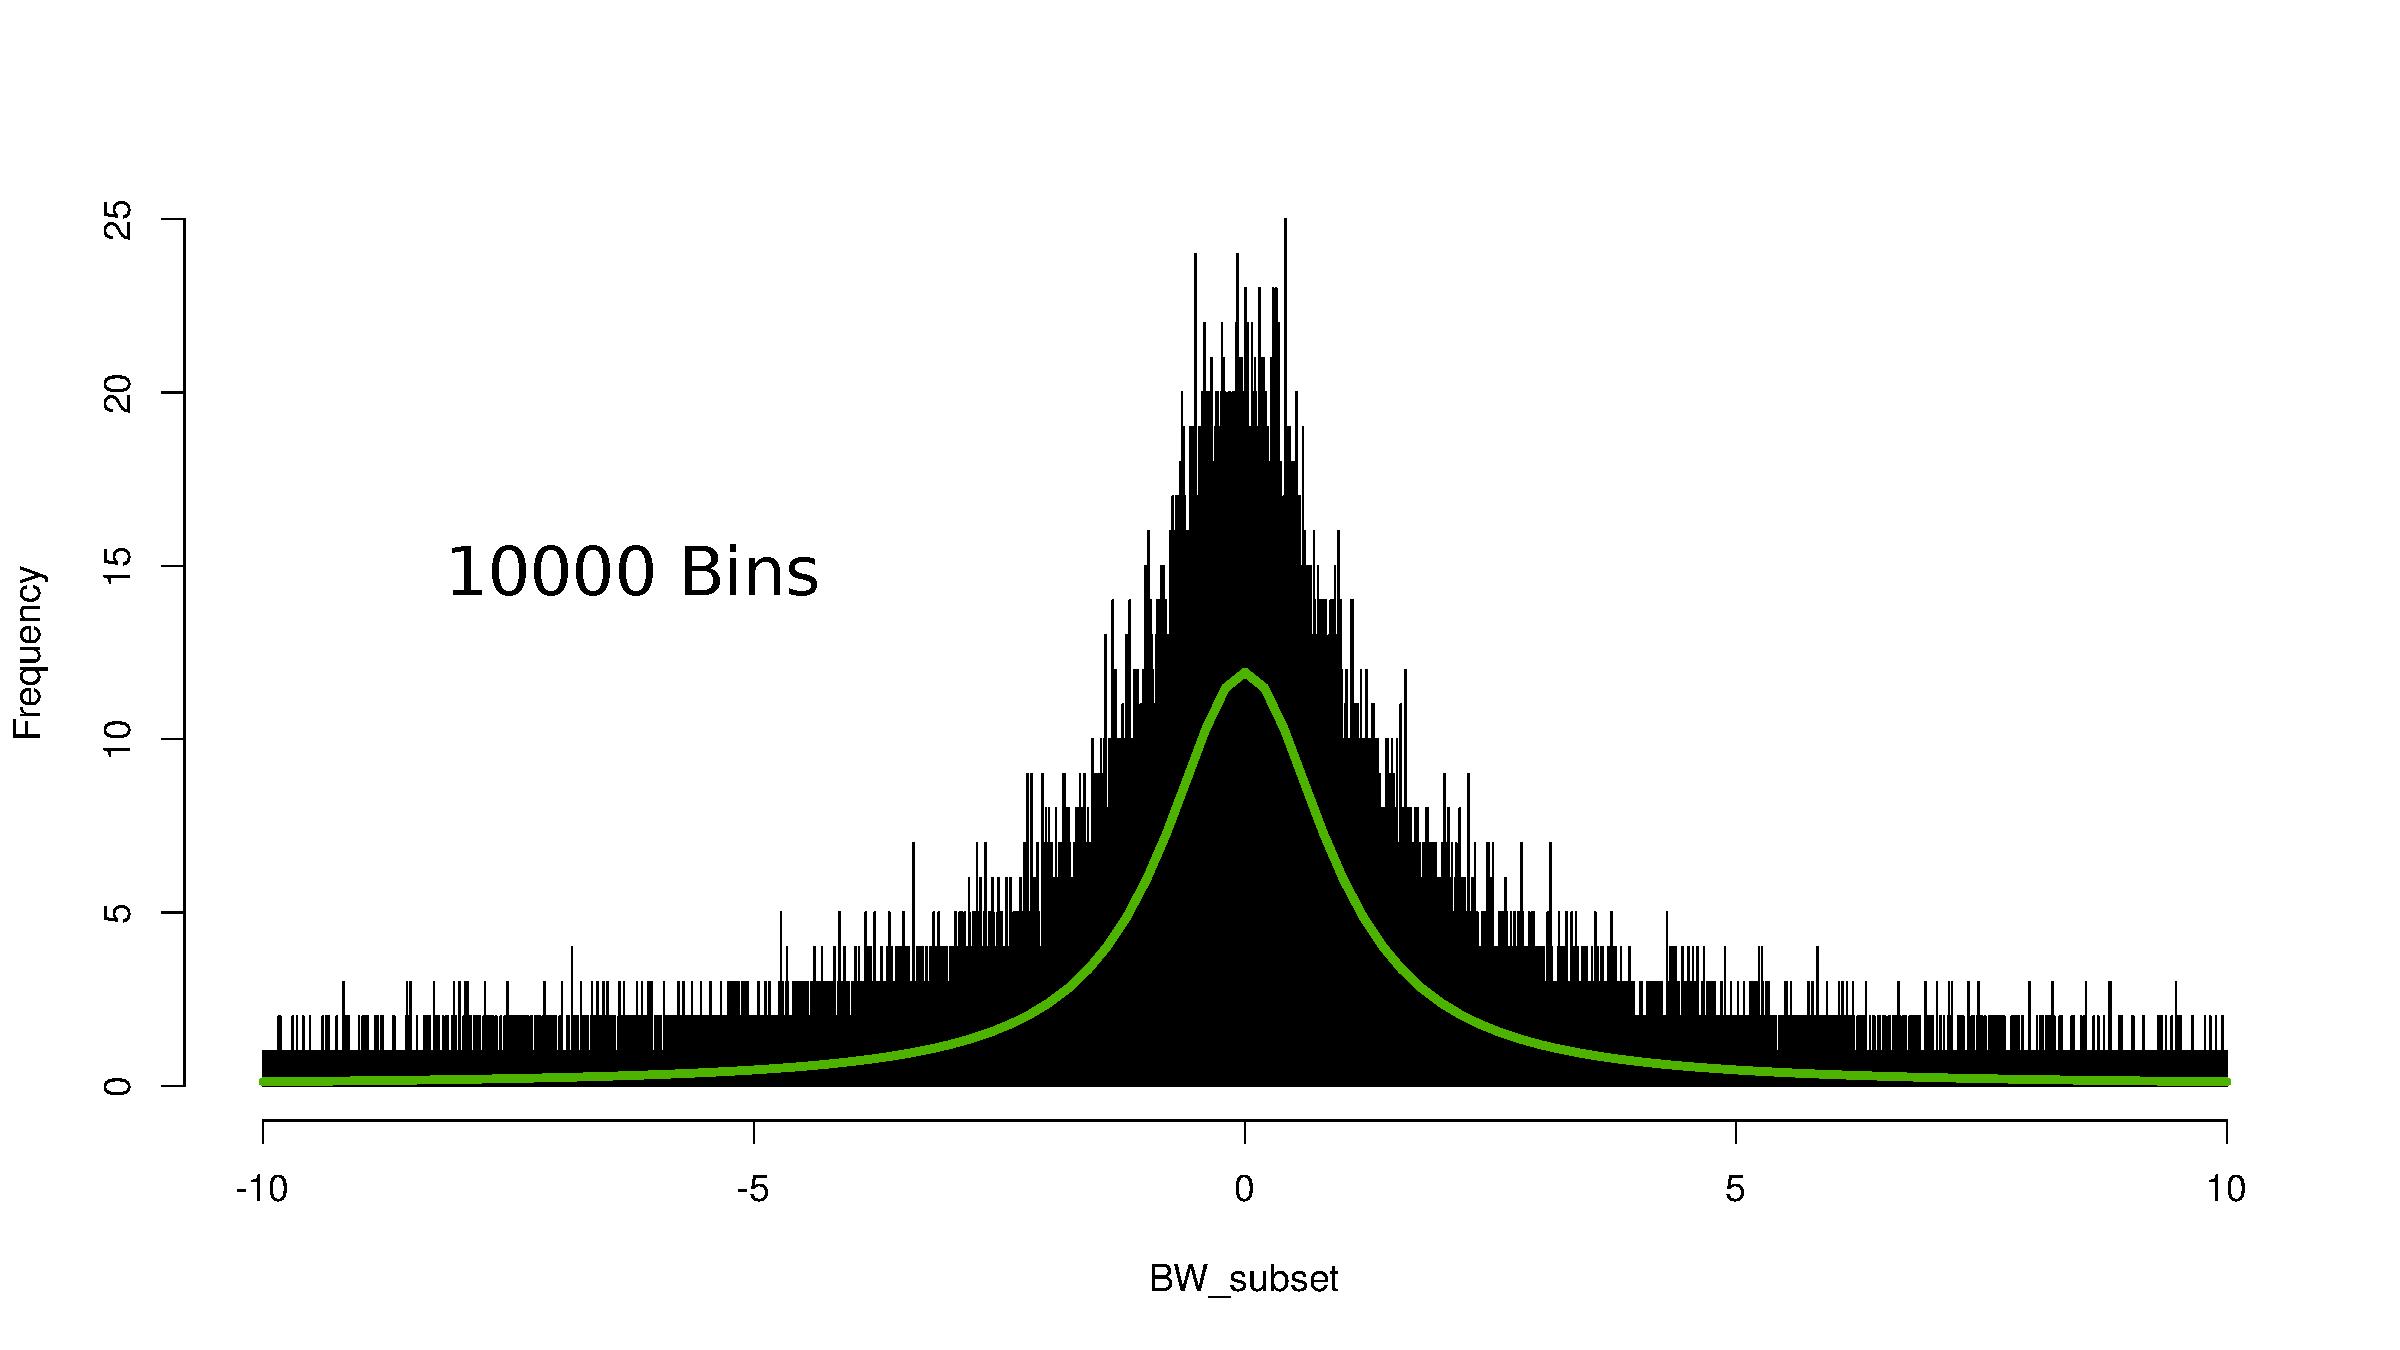
\includegraphics[width = 2.9in]{Immagini/BW_histogram_10000bins.pdf}}
	\label{fig:Breit-Wigner_BINS}
\end{figure}

\begin{figure}
	\centering
	\caption{Istogrammi generati utilizzando $500$ bin, ma con differente numero di eventi totali.}
	\subfloat[]{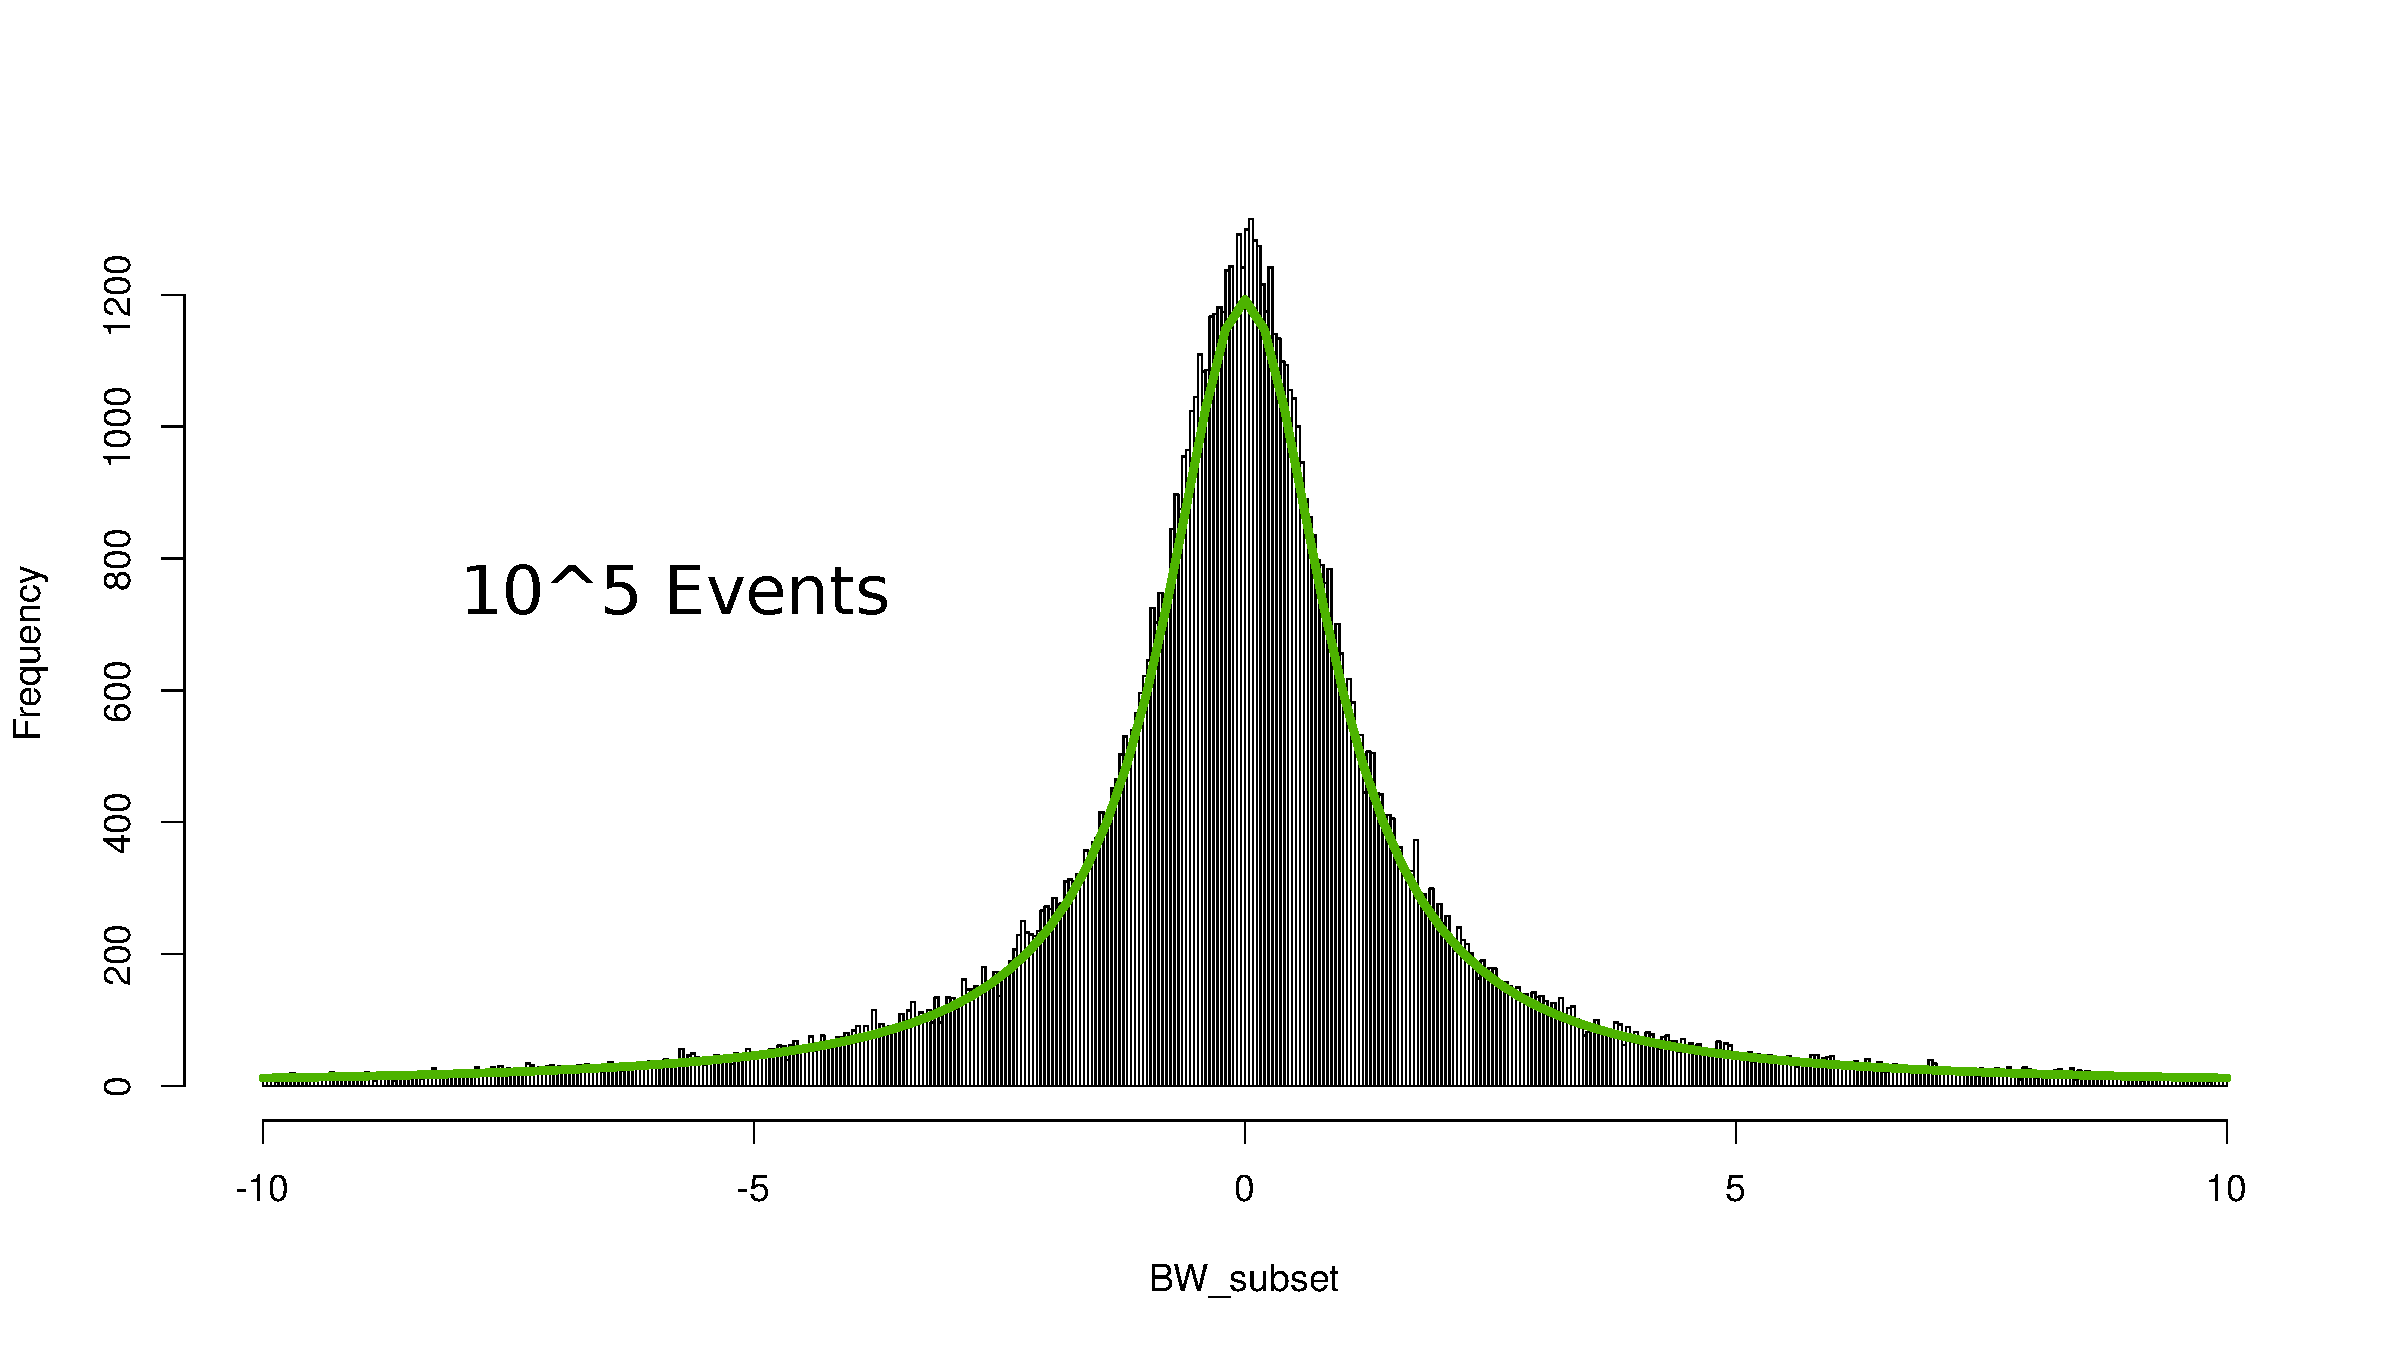
\includegraphics[width = 6in]{Immagini/BW_histogram_E5.pdf}} \\
	\subfloat[]{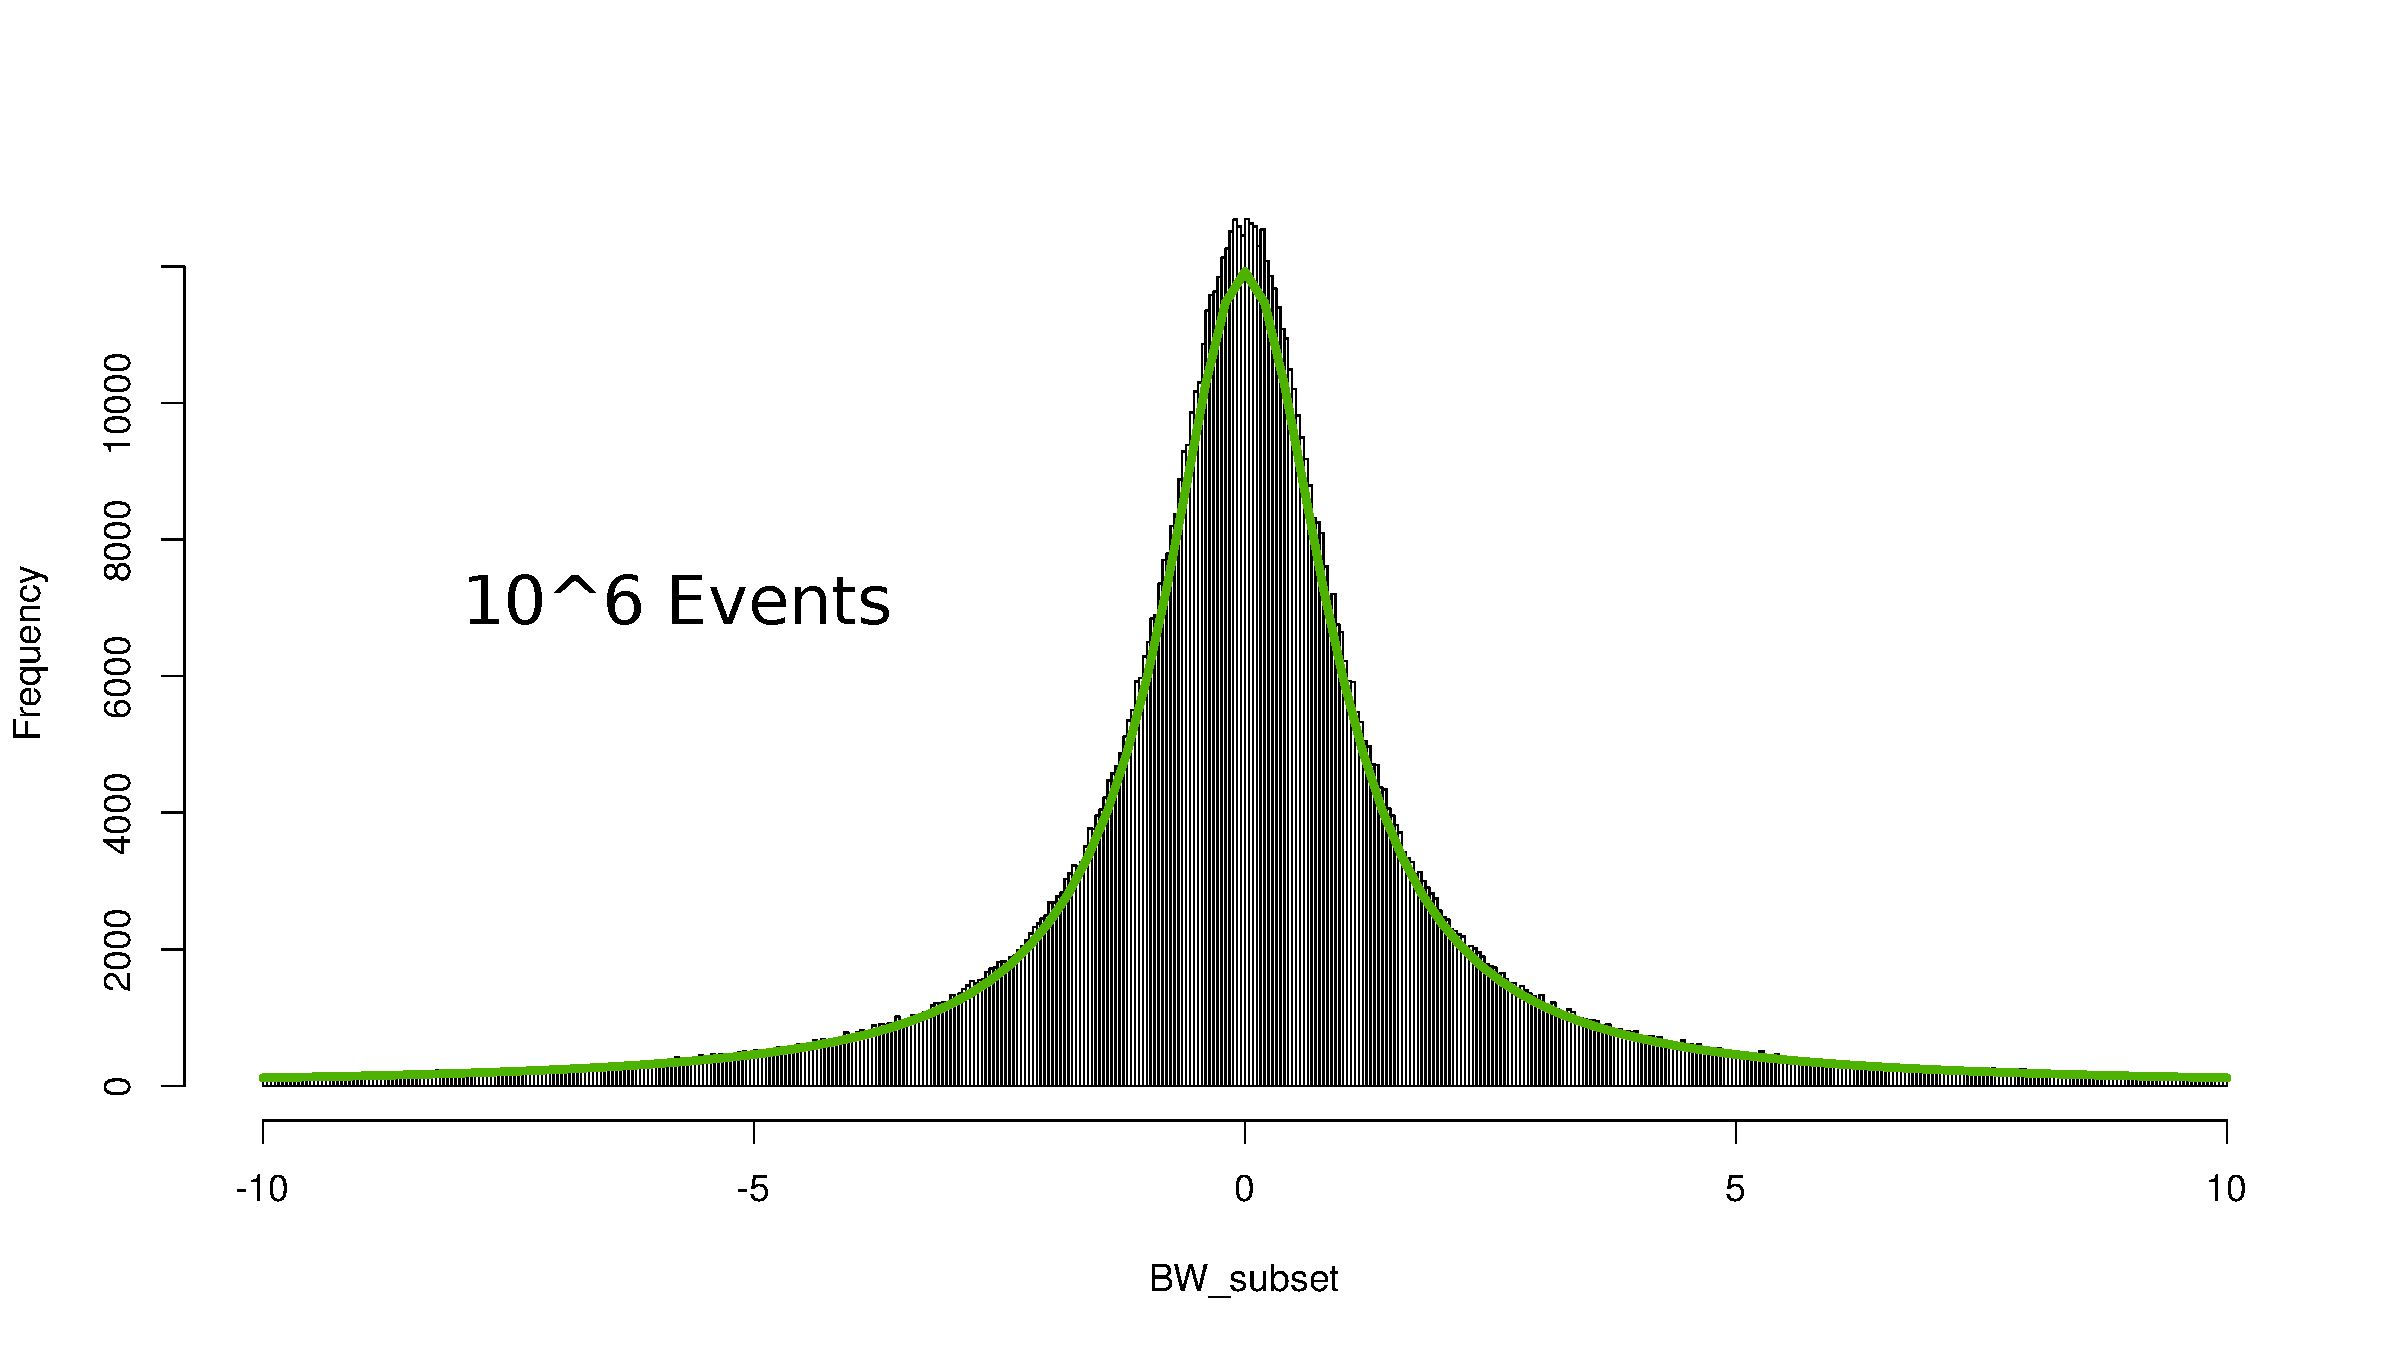
\includegraphics[width = 6in]{Immagini/BW_histogram_E6.pdf}}
	\label{fig:Breit-WIgner_N}
\end{figure}

\newpage

\noindent Passiamo adesso al problema dell'implementazione e del test di un generatore casuale uniforme. L'algoritmo che adotteremo è ad oggi considerato lo standard minimo in termini di prestazioni della sequenza pseudo-random generata: si tratta del \emph{Linear Congruential Method}, nella formulazione di Lewis, Goodman e Miller (Minimal Standard LCG).\footnote{Si vedano ad esempio le \emph{lecture notes}: \url{https://people.smp.uq.edu.au/DirkKroese/mccourse.pdf}.}\\

\vfill

\noindent In sostanza si tratta di generare la sequenza secondo la seguente formula ricorsiva:

\begin{align*}
X&_0 = s\\
X&_{t+1} = (aX_t + b) \mathop{\mathrm{mod}}c\\
U&_{t} = \frac{r}{c} \cdot X_t
\end{align*}

\noindent dove $a$, $b$, $c$ e $s$, sono numeri interi tali che

$$ a, b, s \in \{0, 1, \dots, c-1\},$$

\noindent e i numeri $\{U\}$ così costruiti risultano distribuiti uniformemente nell'intervallo aperto\footnote{Le ragioni per cui tutti i generatori di numeri pseudo-casuali lavorano su intervalli aperti sono di natura computazionale. In sostanza se qualcuno degli $U$ assumesse esattamente uno dei valori estremi si dovrebbero affrontare fastidiosi problemi numerici nell'implementazione di gran parte degli algoritmi che fanno uso di tali generatori.} $]0,r[$. Si ricordi che il risultato dell'operazione binaria $q\mathop{\mathrm{mod}}d$ è il resto della divisione di $q$ per $d$.\\

\vfill

\noindent In generale la qualità della sequenza generata dipende dai valori assegnati ai vari parametri (escluso il \emph{"seme"} $s$), e i dettagli comportano un notevole livello di complicazione matematica.\\

\vfill

\noindent  La scelta del Minimal Standard LCG

\begin{align*}
a &= 7^5\\
b &= 0\\
c &= 2^{31}-1\\
\end{align*}

\noindent pur garantendo buone proprietà di indipendenza alla sequenza $\{U\}$, risulta in un periodo di sole $(2^{31}-2)$ iterazioni, ormai inadeguato per molte applicazioni d'interesse. L'adozione qui di questo metodo è dunque motivata dalla sola semplicità di implementazione dell'algoritmo.\\

\vfill

\noindent La possibilità di scegliere semi diversi per diverse simulazioni è molto importante perché permette di ottenere sequenze indipendenti e quindi di combinare statisticamente i risultati ottenuti.\footnote{Nei metodi Montecarlo applicati alla fisica statistica, ad esempio, risulta spesso più utile combinare più simulazioni con sequenze "relativamente brevi" che generare una sola sequenza complessiva. Ciò è dovuto ai processi di minimizzazione coinvolti, che rischiano di rimanere "intrappolati" in minimi locali delle funzioni considerate. Si consulti ad esempio \href{https://www.elsevier.com/books/understanding-molecular-simulation/frenkel/978-0-12-267351-1}{\textsl{"Understanding Molecular Simulation"}} di Frenkel e Smit (Elsevier 2001).} Nel nostro caso tuttavia ci limiteremo a produrre una sola sequenza, impostando $s=1$: la sequenza risultante è riportata in Figura~\ref{fig:LCGhist} sottoforma di istogramma delle frequenze dei primi $10^5$ numeri generati.\\

\vfill

\begin{figure}
	\centering
	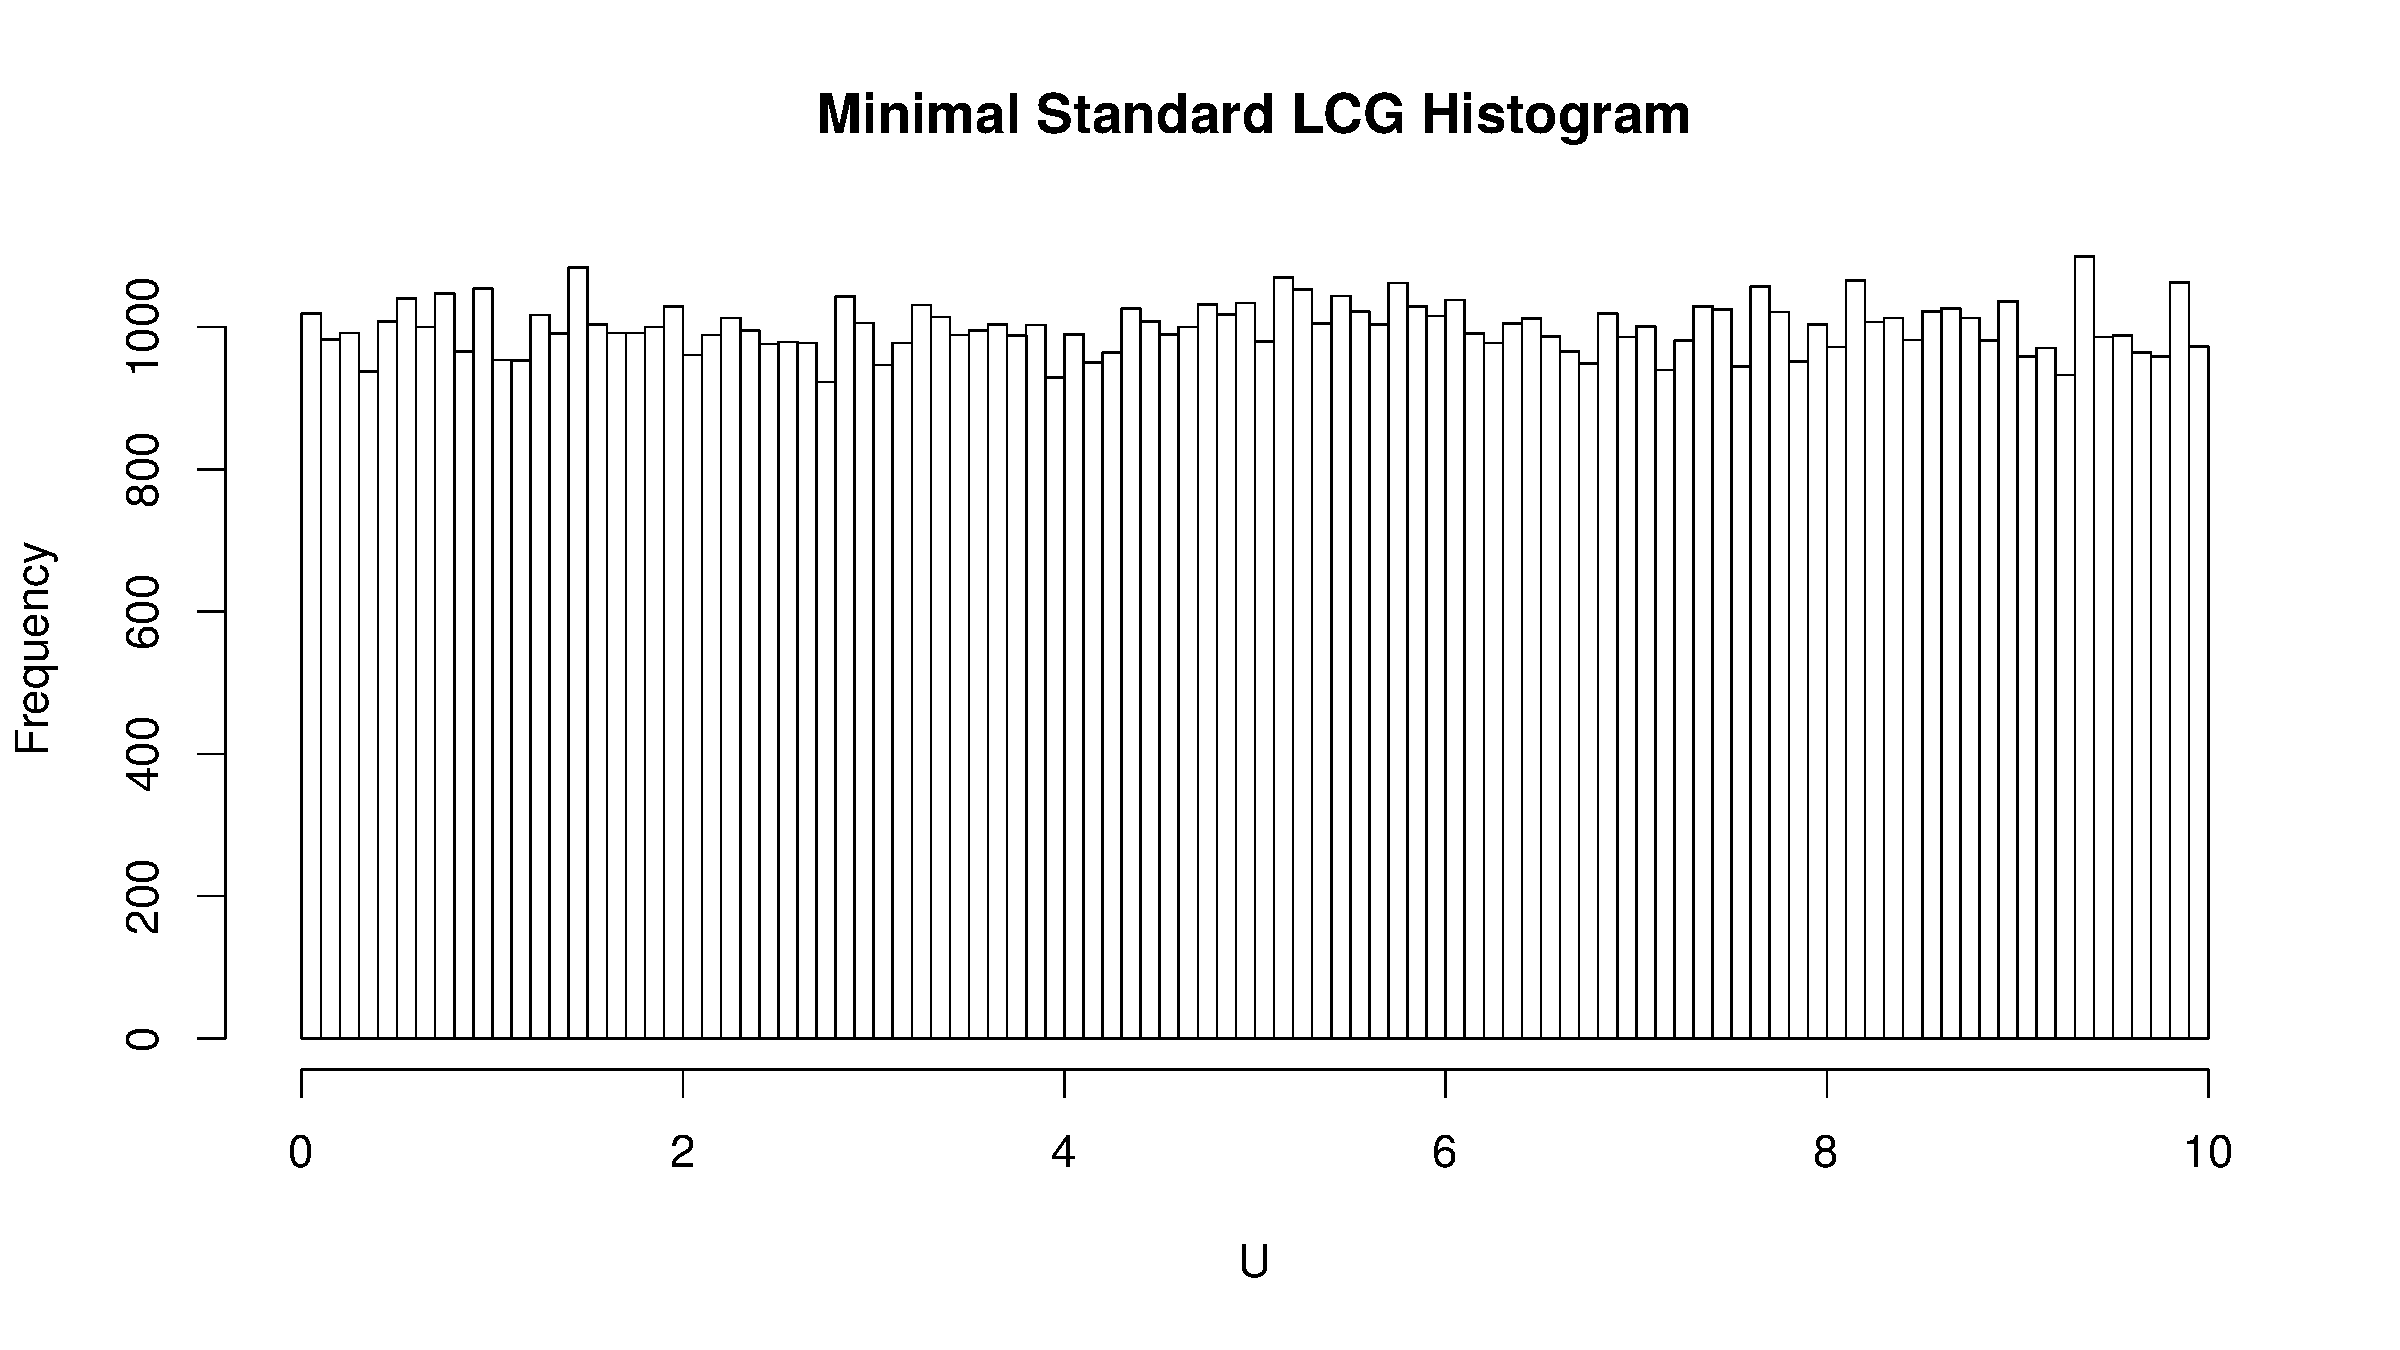
\includegraphics[width=\textwidth, trim={0 3cm 0 0}, clip]{Immagini/LCG_histogram.pdf}
	\caption{Istogramma di $10^5$ numeri generati con algoritmo Minimal Standard LCG, nell'intervallo $]0,10[$.}
	\label{fig:LCGhist}
\end{figure}

\newpage

\begin{lstlisting}[language=R, style=Rstyle, caption=\texttt{R} code for Minimal Standard LCG, xleftmargin=.02\textwidth]
# Defining Minimal Standard parameters for LCG
a = 7^5
b = 0
c = 2^31-1

# Entering user's choice parameters (length of sequence, interval radius and seed)
n = 10^5
r = 10
s = 1
	
# Inizializing recursive vectors
x = numeric(length = n)
u = numeric(length = n)
x[1] = s

# Recursive cycle
t = 1
while(t < n)
{		u[t] = x[t] * r/c; 						#Normalizing the output
		x[t+1] = (a*x[t] + b) %% c;		#Recursive action (%% is R syntax for mod)
		t = t+1
};  u[t] = x[t] * r/c 
	
# Saving a histogram plot of {u}
cairo_pdf('LCG_histogram.pdf', width = 16, height = 9, pointsize = 22)
LCG_hist = hist(u, breaks = n/1000)
LCG_hist$name = 'Minimal Standard LCG Histogram'
LCG_hist$ylab = 'Frequency'
plot(LCG_hist,  ylab=LCG_hist$ylab, main=LCG_hist$name)
dev.off()
\end{lstlisting}

\bigskip

\noindent Il primo test cui possiamo sottoporre i numeri pseudo-casuali appena generati è senz'altro un calcolo della media e della varianza campionarie. Questi sono difatti degli stimatori non distorti per cui ci aspettiamo che,  al crescere del numero di estrazioni, convergano ai "valori veri" della distribuzione di probabilità che si vuole simulare.\\

\noindent Cominciamo dunque ricordando le espressioni che definiscono la media e la varianza di una distribuzione uniforme nell'intervallo $[x,y]$:

\begin{align*}
\mathrm{E}[u(x,y)] =  \frac{x+y}{2} &=: \mu(x,y)\\ \\
\mathrm{Var}[u(x,y)] = \frac{(y-x)^2}{12} &=: \sigma^2(x,y)\\
\end{align*}

\noindent per cui nel nostro caso $\mu(0,10)=5$ e $\sigma(0,10) = 8.\bar{3}$ saranno i valori di riferimento.\\

\noindent Per quanto riguarda gli stimatori campionari, essi sono definiti come segue:

\begin{align*}
\hat{\mu}(n) &:= \frac{1}{n}\sum_{t=0}^{n-1} U_t \\ \\
\hat{\sigma}^2(n) &:= \frac{1}{n-1}\sum_{t=0}^{n-1} \left(U_t - \hat{\mu}(n)\right)^2\\
\end{align*}

\noindent Dal nostro campione otteniamo risultati soddisfacenti:

\bgroup
\def\arraystretch{1.5}
\begin{center}
\begin{tabular}{l||c|c|c}
	$n=10^5$&valore vero&valore stimato&errore relativo $\!\times\,10^{-3}$\\ \hline
	media&$5$&$5.002841\dots$&$0.568\dots $\\
	varianza&$8.\bar{3}$&$8.319576\dots$&$1.651\dots$\\	
\end{tabular}
\end{center}
\egroup

\noindent da cui deduciamo che il generatore riproduce bene tali proprietà della distribuzione uniforme.\\

\begin{lstlisting}[language=R, style=Rstyle, caption= \texttt{R} code for computing non-biased variance and mean predictors, xleftmargin=.02\textwidth]
# Assuming to have a vector u[t], with t = 1,...,n and uniform distributed in [0,r]

	# Sample Mean
	sm = 0
	for (t in seq(1, n, by = 1))
		{ sm = sm + u[t] / n }
	
	# Sample Variance
	ss = 0
	for (t in seq(1, n, by = 1))
		{ ss = ss + (u[t] - sm)^2 / (n-1) }
		
	# Displaying results and relative deviation from 'true values'
	true_media = r/2;		true_varianza = r^2/12;
	media = sm;		varianza = ss
	e_media = abs(media - true_media)/true_media
	e_varianza = abs(varianza - true_varianza)/true_varianza
	media; varianza; e_media; e_varianza;
\end{lstlisting}

\noindent Tuttavia il controllo delle sole media e varianza campionarie non può davvero garantire la bontà di una realizzazione campionaria della densità da simulare. Procederemo dunque alla costruzione di opportuni \emph{test d'ipotesi} le cui ipotesi nulle consistano nell'assumere che la sequenza generata segua effettivamente la distribuzione desiderata. Qualora i \emph{p-value} ottenuti consentano di rifiutare tale ipotesi potremmo dire di aver rilevato un problema statisticamente significativo nella sequenza generata.

\begin{description}\label{PearsonTest}
	\item[\quad\quad\! Test "chi-quadro" alla Pearson]\quad\\
	\noindent Il primo test considerato è basato sulla cosiddetta statistica \emph{"chi-quadro"}, definita come:
	
	\begin{equation*}
	\chi_{_{k-1}}^2 = \sum_{i=1}^{k} \frac{(o_i - e_i)^2}{e_i},
	\end{equation*}
	
	\noindent dove $o_i$ e $e_i$ sono le frequenze rispettivamente osservata e attesa per l'evento $E_i$, e $k-1$ sono detti essere i \emph{gradi di libertà} della statistica. Dunque nel nostro caso, diviso l'intervallo $]0,10[$ in $k$ bin, valuteremo lo scarto quadratico normalizzato tra le frequenze istogrammate dalla sequenza generata e il valore atteso di $(10^5 / k)$ eventi su ciascun bin. Evidentemente quanto più la sequenza estratta sarà aderente alla distribuzione uniforme, tanto più il valore ottenuto per la statistica $\chi^2$ sarà tendente a zero. Tra i vari test che possono essere implementati su tale statistica utilizzeremo quello di \emph{Pearson}, nativamente incorporato in \texttt{R}\footnote{Comando \texttt{chisq.test}: \url{https://stat.ethz.ch/R-manual/R-devel/library/stats/html/chisq.test.html}}, e ben adatto al caso in analisi\footnote{Il test di Pearson presenta problemi qualora alcune delle frequenze attese siano molto piccole, per cui per distribuzioni con "lunghe code" potrebbe risultare inutilizzabile. Di certo una densità uniforme non presenta criticità in tal senso.}.\smallskip

	\noindent Lavorando con tre diversi istogrammi dei nostri $10^5$ campioni abbiamo ottenuto i seguenti risultati:
	
	\bgroup
	\def\arraystretch{1.5}
	\begin{center}
		\begin{tabular}{c|c}
			Number of bins & Pearson's \emph{p-value}\\ \hline\hline
			500 & 0.94475363037911164\\
			750 & 0.86939873721667693\\
			1000 & 0.85937070391061714\\
		\end{tabular}
	\end{center}
	\egroup
	
	\noindent I \emph{p-value} ottenuti sono tali per cui fissato un qualsiasi grado ragionevole di significatività non possiamo rigettare l'ipotesi di una sequenza distribuita uniformemente: il generatore implementato ha superato il test di Pearson.
	
	\item[\quad\quad\! Test di Kolmogorov-Smirnov]\quad\\
	\noindent Un altro test d'ipotesi appropriato alla nostra situazione è quello di Kolmogorv e Smirnov (KS), basato sulla funzione cumulante $F(x)$. L'ipotesi nulla sarà dunque formulata in termini di $F(x)$ e della sua candidata realizzazione campionaria $\hat{F}_n(x)$: $H_0 = \{\hat{F}_n(x) = F(x), \,\forall x\}$. Il test è ben definito solo se $F(x)$ è continua su tutto il dominio.
	La statistica di riferimento è molto semplice: si tratta dello scarto massimo tra cumulante teorica e sua realizzazione campionaria $D_n = \max |\hat{F}_n(x) - F(x)|$, sul cui valore viene stabilito un \emph{decision boundary} oltre il quale rifiutare $H_0$. A tale valore di taglio è associata una significatività $\alpha$, secondo le formule:
	
	\begin{align*}
	D_n^{^\mathrm{cut}} &= \frac{\lambda_\alpha}{\sqrt{n}},\\
	1-\alpha &= \sum_{k=-\infty}^{\infty} (-1)^k \exp\left[-2k^2\lambda_\alpha\right].
	\end{align*}
	
	\noindent Anche il test KS è nativamente implementato in \texttt{R}\footnote{Comando \texttt{ks.test}: \url{https://stat.ethz.ch/R-manual/R-devel/library/stats/html/ks.test.html}} e per i primi 100 numeri della sequenza generata ha restituito: $D_{100} \simeq 0.05954$ e $\lambda_{0.01} \simeq 1.6276$. Dunque avendo $D_{100} < D_{100}^{^\mathrm{cut}} = 0.16276$ possiamo affermare che, fissata una significatività del 1\%, anche il test KS conferma la bontà dal nostro generatore LCG.

\end{description}

\noindent Infine osserviamo che sebbene il superamento dei test d'ipotesi proposti dia una conferma molto solida su quanto la sequenza generata riproduca la distribuzione da simulare, resta ancora la possibilità che una sequenza palesemente deterministica, e quindi affetta da spiacevoli correlazioni, minimizzi molto efficientemente gli scarti sulla $f(x)$ e sulla $F(x)$ che i test vanno a controllare. Per scongiurare questa possibilità si potrebbero ripetere i test molte volte, variando in un grande range la dimensione dei bin utilizzati, ma questo evidentemente implica un grande dispendio di risorse computazionali. Quindi preferiamo affidarci ad un metodo di controllo visivo e immediato per scovare eventuali correlazioni fra coppie di numeri estratti consecutivamente\footnote{Va da sé che andrebbero controllate anche le correlazioni fra numeri estratti non consecutivamente, ma ci aspettiamo che gli effetti di correlazione diminuiscano fortemente al crescere del numero di "passi" che ne separano l'estrazione nell'algoritmo del generatore (purché si stia ben sotto il periodo di ricorrenza!).}: costruiamo uno \emph{scatter-plot} bidimensionale in cui in ascissa sono riportati i numeri estratti ai passi dispari e in ordinata i numeri estratti ai passi pari. Il risultato, visibile in \figurename~\ref{fig:SimulatedWhiteNoise}, non mostra nessun evidente pattern distinguibile da un generico e omogeneo "rumore bianco", per cui possiamo concludere che il generatore non presenta problemi di eccessiva correlazione nella sequenza~prodotta.

\begin{figure}[h!]
	\centering
	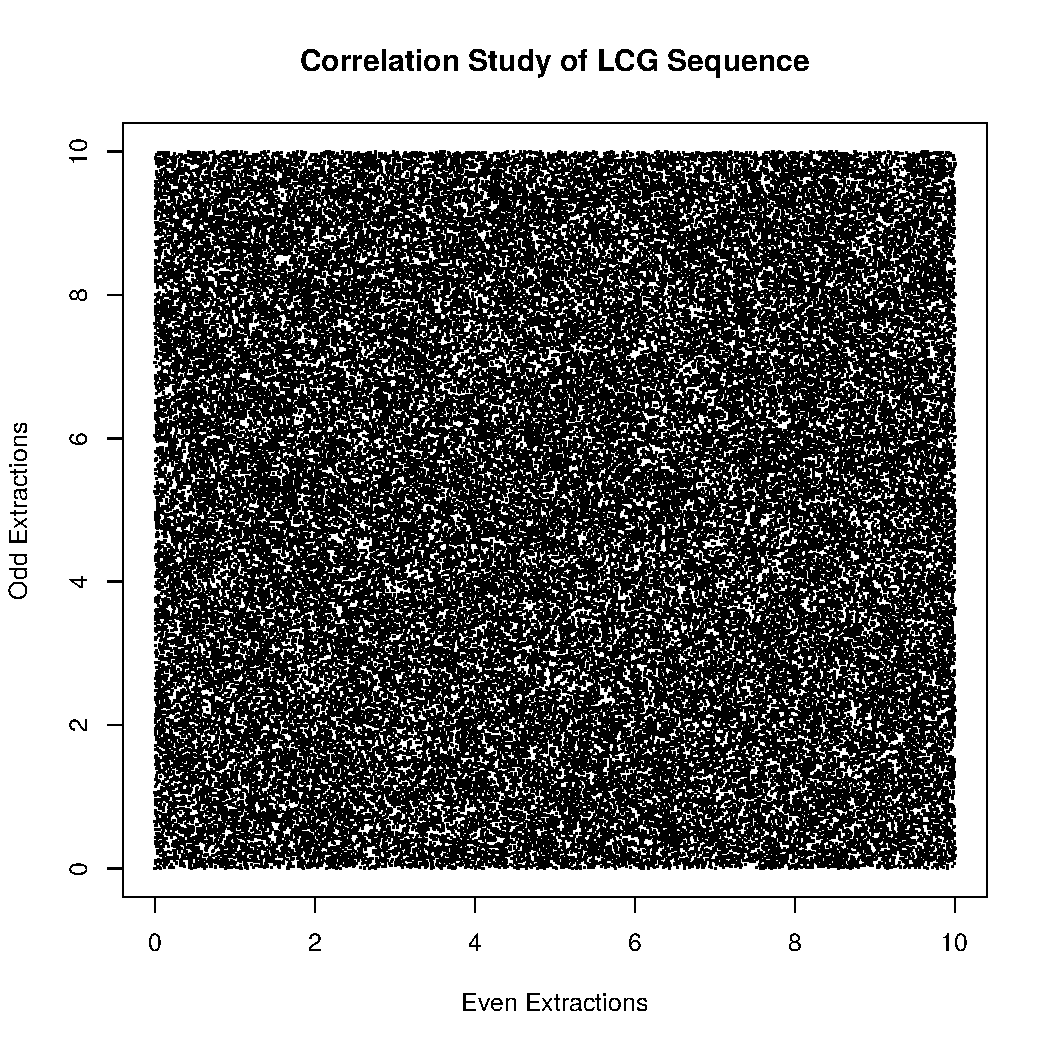
\includegraphics[width=0.55\linewidth, trim={0 0.5cm 0 0cm}, clip]{Immagini/CorrelationStudy}
	\caption{Visualizzazione delle eventuali correlazioni fra numeri estratti consecutivamente dal generatore LCG.}
	\label{fig:SimulatedWhiteNoise}
\end{figure}


\begin{lstlisting}[language=R, style=Rstyle, caption= \texttt{R} code for correlation-study of LCG random sequence]
# Assuming to have a vector u[t], of uniform distributed pseudo-random numbers...
	
	# Subset of "even extrations"
	X = u[c(TRUE,FALSE)] 
	# Subset of "odd extractions"
	Y = u[c(FALSE,TRUE)]
	# Saving a scatter-plot of Y vs X
	cairo_pdf('CorrelationStudy.pdf')
	Xlab = 'Even Extractions'
	Ylab = 'Odd Extractions'
	Title = 'Correlation Study of LCG Sequence'
	plot(X , Y, pch = '.', xlab = Xlab, ylab = Ylab, main = Title)
	dev.off()
\end{lstlisting}

\newpage